% =====================================================================
%  05124710 - Laboratory in FPGA -- Tel Aviv University
%  Experiment 7 -- Snake Game -- Final Report
%  Authors: Saleh Khalil, Mahmood Isteteh
%
%  This folder is self-contained: all images are under figures/ and
%  tau.png, all sources under src/. Upload the whole LaTeX/ folder to
%  Overleaf and compile with pdfLaTeX.
%
%  >>> FILL IN the two ID numbers in the two commands right below. <<<
% =====================================================================
\documentclass[11pt,a4paper]{article}

\newcommand{\IDone}{\texttt{[213310485]}}   % <-- Saleh Khalil, ID
\newcommand{\IDtwo}{\texttt{[ID2]}}   % <-- Mahmood Isteteh, ID
\newcommand{\youtubelink}{https://youtu.be/REPLACE-ME}  % <-- paste your YouTube demo URL here

\usepackage[margin=2.4cm]{geometry}
\usepackage{graphicx}
\usepackage{xcolor}
\usepackage{booktabs}
\usepackage{caption}
\usepackage{float}
\usepackage{listings}
\usepackage{fancyhdr}
\usepackage[colorlinks=true, linkcolor=blue!50!black, urlcolor=blue!50!black]{hyperref}

\graphicspath{{./}}

% ------------- header / footer -------------
\pagestyle{fancy}
\fancyhf{}
\fancyhead[L]{\small 05124710 -- Laboratory in FPGA}
\fancyhead[R]{\small Experiment 7 -- Snake Game}
\fancyfoot[C]{\small\thepage}
\renewcommand{\headrulewidth}{0.4pt}

% ------------- placeholder box for missing results -------------
\newcommand{\placeholderbox}[2]{%
  \begin{center}
    \setlength{\fboxsep}{10pt}\setlength{\fboxrule}{1pt}
    \fbox{\begin{minipage}[c][#1][c]{0.88\textwidth}\centering
      \textbf{\textcolor{red!60!black}{[PLACEHOLDER -- RESULT NOT YET AVAILABLE]}}\\[6pt]
      \small #2
    \end{minipage}}
  \end{center}}

% ------------- Verilog listings -------------
\definecolor{codegreen}{rgb}{0.0,0.45,0.0}
\definecolor{codegray}{rgb}{0.5,0.5,0.5}
\definecolor{codeblue}{rgb}{0.1,0.15,0.6}
\lstset{
  language=Verilog,
  basicstyle=\ttfamily\footnotesize,
  keywordstyle=\color{codeblue}\bfseries,
  commentstyle=\color{codegreen},
  stringstyle=\color{codegray},
  numbers=left,
  numberstyle=\tiny\color{codegray},
  numbersep=6pt,
  frame=single,
  breaklines=true,
  postbreak=\mbox{\textcolor{codegray}{$\hookrightarrow$}\space},
  tabsize=4,
  showstringspaces=false,
  columns=fullflexible,
  keepspaces=true
}

\sloppy

\begin{document}

% =====================================================================
%  COVER PAGE
% =====================================================================
\begin{titlepage}
  \centering
  
\includegraphics[width=0.38\textwidth]{tau.png}\\[0.8cm]
  {\Large Tel Aviv University}\\[0.15cm]
  {\large The Iby and Aladar Fleischman Faculty of Engineering}\\[1.6cm]

  {\large 05124710 -- Laboratory in FPGA}\\[0.4cm]
  {\large Experiment 7 -- Final Report}\\[1.2cm]

  \rule{0.72\textwidth}{1pt}\\[0.55cm]
  {\Huge\bfseries Snake Game}\\[0.55cm]
  \rule{0.72\textwidth}{1pt}\\[2.0cm]

  {\large\bfseries Authors}\\[0.5cm]
  \begin{tabular}{ll}
    \toprule
    \textbf{Name} & \textbf{ID} \\
    \midrule
    Saleh Khalil    & \ 213310485 \\
    Mahmood Isteteh & \ 214032682 \\
    \bottomrule
  \end{tabular}\\[2.2cm]

  {\large \today}
  \vfill
\end{titlepage}

% =====================================================================
%  TABLE OF CONTENTS
% =====================================================================
\tableofcontents
\newpage

% =====================================================================
\section{Introduction}
% =====================================================================
In this experiment we designed and implemented a complete \emph{Snake}
game on the Digilent Basys3 board. The game is
displayed on a computer monitor through the VGA interface, the current
score is shown on the on-board 4-digit 7-segment display, and the player
steers the snake with a PS/2 keyboard.

\subsection{Game rules}
The playing field is a $100\times75$ grid of $8\times8$-pixel cells on an
$800\times600$ VGA screen. The snake advances one cell per game tick in
the current direction; eating the red food cell makes it grow by one cell
and increments the score, and every food item also makes the game tick
slightly faster. The game ends when the snake hits a wall or its own
body, after which a game-over screen is shown and the game can be
restarted by pressing any key on the keyboard.

% \subsection{Requirements}
% Table~\ref{tab:reqs} maps every requirement of the assignment to the
% place in the design where it is fulfilled.

% \begin{table}[H]
%   \centering\small
%   \caption{Assignment requirements and where they are implemented.}
%   \label{tab:reqs}
%   \begin{tabular}{p{0.42\textwidth}p{0.50\textwidth}}
%     \toprule
%     \textbf{Requirement} & \textbf{Implementation} \\
%     \midrule
%     1a. Visualize the game via VGA &
%       \texttt{VGA\_Interface.v} (sync/scan) + \texttt{Pixel\_Painter.v}
%       (per-pixel color), $800\times600$. \\
%     1b. Snake and food clearly distinguishable &
%       Dark grey body (\texttt{0x444}), darker head (\texttt{0x222}), red
%       food (\texttt{0xF11}) on a two-tone green checkerboard
%       (\texttt{grid\_mapper.v}). \\
%     1c. Sufficient refresh rate &
%       VESA $800\times600$ @ 72\,Hz (50\,MHz pixel clock). \\
%     2a. Score on the 7-segment display &
%       \texttt{Seg\_7\_Display.v} driven by the snake length. \\
%     2b. Score increments when food is eaten &
%       \texttt{score = length} in \texttt{snake.v}; length grows on eat. \\
%     3a. Keyboard control, 4/6/8/5 = left/right/up/down &
%       \texttt{Navigation\_System.v}, scancodes \texttt{6B/74/75/73}. \\
%     3b. No immediate direction reversal &
%       Guarded direction update (e.g.\ LEFT forbidden while RIGHT). \\
%     4a. Game-over on wall / self collision &
%       \texttt{crash} logic in \texttt{snake.v}. \\
%     4b. \textbf{Bonus}: game-over screen &
%       Skull ``YOU DIED'' bitmap screen in \texttt{grid\_mapper.v}; a
%       welcome splash screen was added as well. \\
%     \bottomrule
%   \end{tabular}
% \end{table}

% =====================================================================
% \newpage
\vspace{1cm}
\section{Design Overview}
% =====================================================================
\subsection{High-level block diagram}
Figure~\ref{fig:hier-all} shows the complete desig, dataflow between the blocks and the three testbenches.

\begin{figure}[H]
  \centering
  
\includegraphics[width=\textwidth]{hierarchy_all.png}
  \caption{Full design map}
  \label{fig:hier-all}
\end{figure}


\newpage
\subsection{File inventory}
\begin{table}[H]
  \centering\small
  \caption{All files and their modules}
  \label{tab:files}
  \begin{tabular}{llll}
    \toprule
    \textbf{File} & \textbf{Module} & \textbf{Role} & \textbf{Origin} \\
    \midrule
    \texttt{FA.v}                 & \texttt{FA}                 & 1-bit full adder           & reuse (Lab 1) \\
    \texttt{CSA.v}                & \texttt{CSA}                & conditional sum adder & reuse (Lab 1) \\
    \texttt{Debouncer.v}          & \texttt{Debouncer}          & signal debounce      & reuse (Lab 1) \\
    \texttt{Seg\_7\_Display.v}    & \texttt{Seg\_7\_Display}    & score display        & reuse (Lab 1) \\
    \texttt{Lim\_Inc.v}           & \texttt{Lim\_Inc}           & limited incrementer  & reuse (Lab 2) \\
    \texttt{Ps2\_Interface.v}     & \texttt{Ps2\_Interface}     & keyboard interface   & reuse (Lab 5) \\
    \texttt{VGA\_Interface.v}     & \texttt{VGA\_Interface}     & VGA interface        & reuse (Lab 6) \\
    \midrule
    \texttt{game\_tick.v}         & \texttt{Game\_Tick}         & movement speed      & new \\
    \texttt{snake.v}              & \texttt{Snake}              & game core            & new \\
    \texttt{farmer.v}             & \texttt{farmer}             & food generator       & new \\
    \texttt{Pixel\_Painter.v}     & \texttt{Pixel\_Painter}     & rendering            & new \\
    \texttt{grid\_mapper.v}       & \texttt{GridMapper}         & grid rendering         & new \\
    \texttt{snake\_game\_tb.v}    & \texttt{snake\_game\_tb}    & integration testbench & new \\
    \texttt{farmer\_tb.v}         & \texttt{farmer\_tb}         & farmer testbench        & new \\
    \texttt{tick\_tb.v}           & \texttt{tick\_tb}           & dynamic tick testbench        & new \\
    \texttt{Navigation\_System.v} & \texttt{Navigation\_System} & direction control    & new \\
    \texttt{snake\_game.v}        & \texttt{snake\_game}        & top level            & new \\
    \midrule
    \texttt{task3.xdc}        & \texttt{-}        & Constraints            & new \\
    \bottomrule
  \end{tabular}
\end{table}




% \subsection{How the modules interact}
% The design is a single pipeline from the keyboard to the monitor, with
% two ``generator'' blocks feeding the core:

% \begin{enumerate}
%   \item \texttt{Ps2\_Interface} deserializes PS/2 frames from the
%         keyboard into a \texttt{scancode} plus a one-clock
%         \texttt{keyPressed} pulse.
%   \item \texttt{Navigation\_System} translates scancodes into a 2-bit
%         direction \texttt{dir}, rejecting $180^{\circ}$ reversals.
%   \item \texttt{Game\_Tick} produces the movement strobe \texttt{tick}
%         ($\approx$7\,Hz at reset) and shortens the period as the score
%         grows -- the game gets faster the longer the snake is.
%   \item \texttt{snake} (the core) keeps the body coordinates, advances
%         the head on every tick, detects wall/self collisions, grows when
%         food is eaten and outputs the score. Internally it instantiates
%         \texttt{farmer}, the LFSR-based food generator.
%   \item \texttt{Pixel\_Painter} + \texttt{GridMapper} convert the VGA
%         scan coordinates into a grid-cell query towards \texttt{snake}
%         (``is this cell body / head / food?'') and answer with the pixel
%         color for the current screen (welcome / play / game over).
%   \item \texttt{VGA\_Interface} generates sync and scan coordinates and
%         drives the RGB pins; \texttt{Seg\_7\_Display} shows the score;
%         \texttt{Debouncer} cleans the centre push-button into a reset
%         pulse.
% \end{enumerate}



% =====================================================================
\vspace{1cm}
\section{Top-Level Integration}
% =====================================================================
% \begin{figure}[H]
%   \centering
%   
\includegraphics[width=\textwidth]{hierarchy_snake_game_snake_game_tb.png}
%   \caption{The top-level block and its integration testbench highlighted.}
%   \label{fig:hier-top}
% \end{figure}
% \placeholderbox{5cm}{The top-level block and its integration testbench highlighted.}

\subsection{\texttt{snake\_game.v} -- top level}
\textbf{Purpose.} Top module file: it holds no logic of its own, 
only the module instantiations and the wires all modules together.
\begin{table}[H]
  \centering\small
  \caption{\texttt{snake\_game} ports}
  \begin{tabular}{lllp{0.45\textwidth}}
    \toprule
    \textbf{Port} & \textbf{Dir} & \textbf{Width} & \textbf{Description} \\
    \midrule
    \texttt{clk}      & in  & 1 & 100\,MHz system clock (pin W5). \\
    \texttt{rst}      & in  & 1 & Centre button, active high (U18). \\
    \texttt{PS2Clk}   & in  & 1 & Keyboard clock (C17). \\
    \texttt{PS2Data}  & in  & 1 & Keyboard data (B17). \\
    \texttt{vgaRed/Green/Blue} & out & $3\times4$ & VGA color channels. \\
    \texttt{Hsync}, \texttt{Vsync} & out & 1 & VGA synchronisation. \\
    \texttt{a\_to\_g}, \texttt{an}, \texttt{dp} & out & 7/4/1 & 7-segment display. \\
    \bottomrule
  \end{tabular}
\end{table}

\newpage
\subsection{IO modules - under \texttt{snake\_game.v}}
Of the eight instantiated modules, four are dedicated to moving data on
and off the board: the keyboard, the VGA monitor, the 7-segment display
and the reset button. The remaining four hold the actual game logic and
are covered in the next subsection.

\begin{figure}[H]
  \centering
  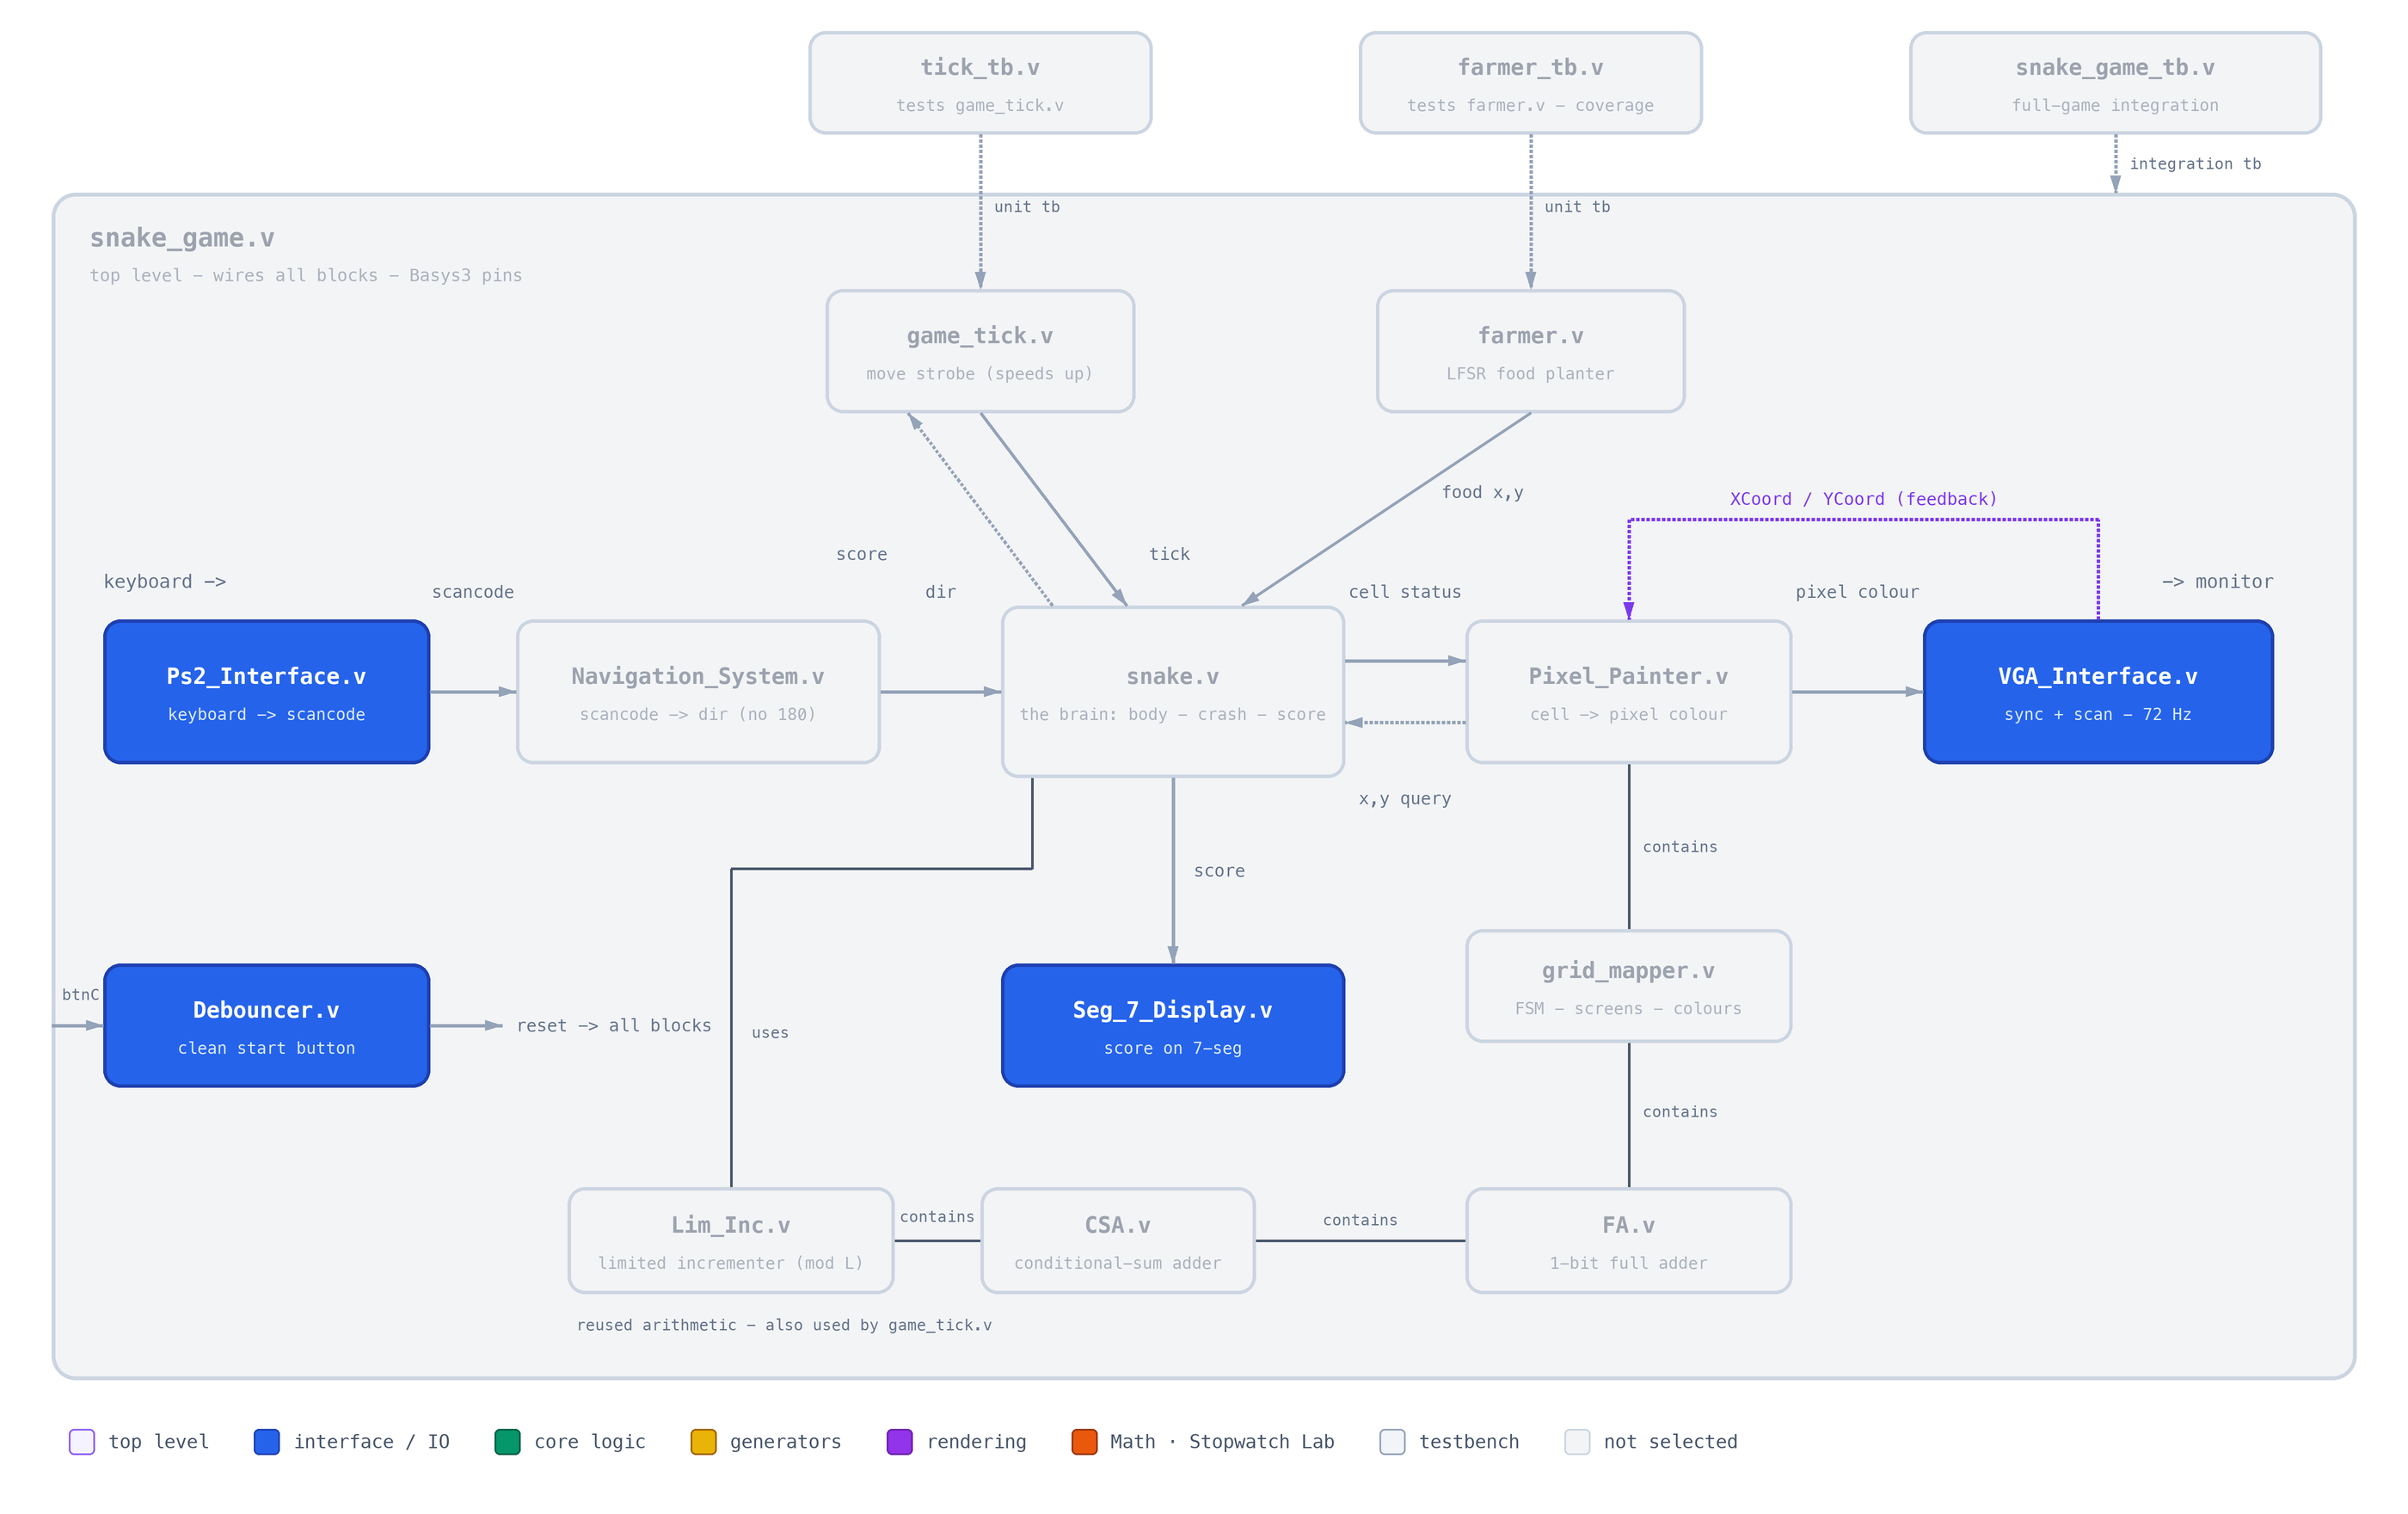
\includegraphics[width=\textwidth]{hierarchy_IO.png}
  \caption{IO modules highlighted.}
  \label{fig:hier-io}
\end{figure}

\begin{itemize}
  \item \textbf{\texttt{Ps2\_Interface.v}} -- Receives PS/2 keyboard frames
    and outputs the make scancode with a single-clock \texttt{keyPressed}.
  \item \textbf{\texttt{Debouncer.v}} -- Converts the bouncy centre
    push-button into a single one-clock reset pulse.
  \item \textbf{\texttt{VGA\_Interface.v}} -- Generates VGA signals for
    $800\times600$ @ 72\,Hz display, drives the RGB pins with the color
    supplied by the \texttt{Pixel\_Painter.v} module, and exports the scan coordinates.
  \item \textbf{\texttt{Seg\_7\_Display.v}} -- Shows the 2-digit score supplied by the \texttt{Snake.v} module on the 7-segment display.
\end{itemize}

% \subsubsection{Internal logic modules}

% \begin{figure}[H]
%   \centering
%   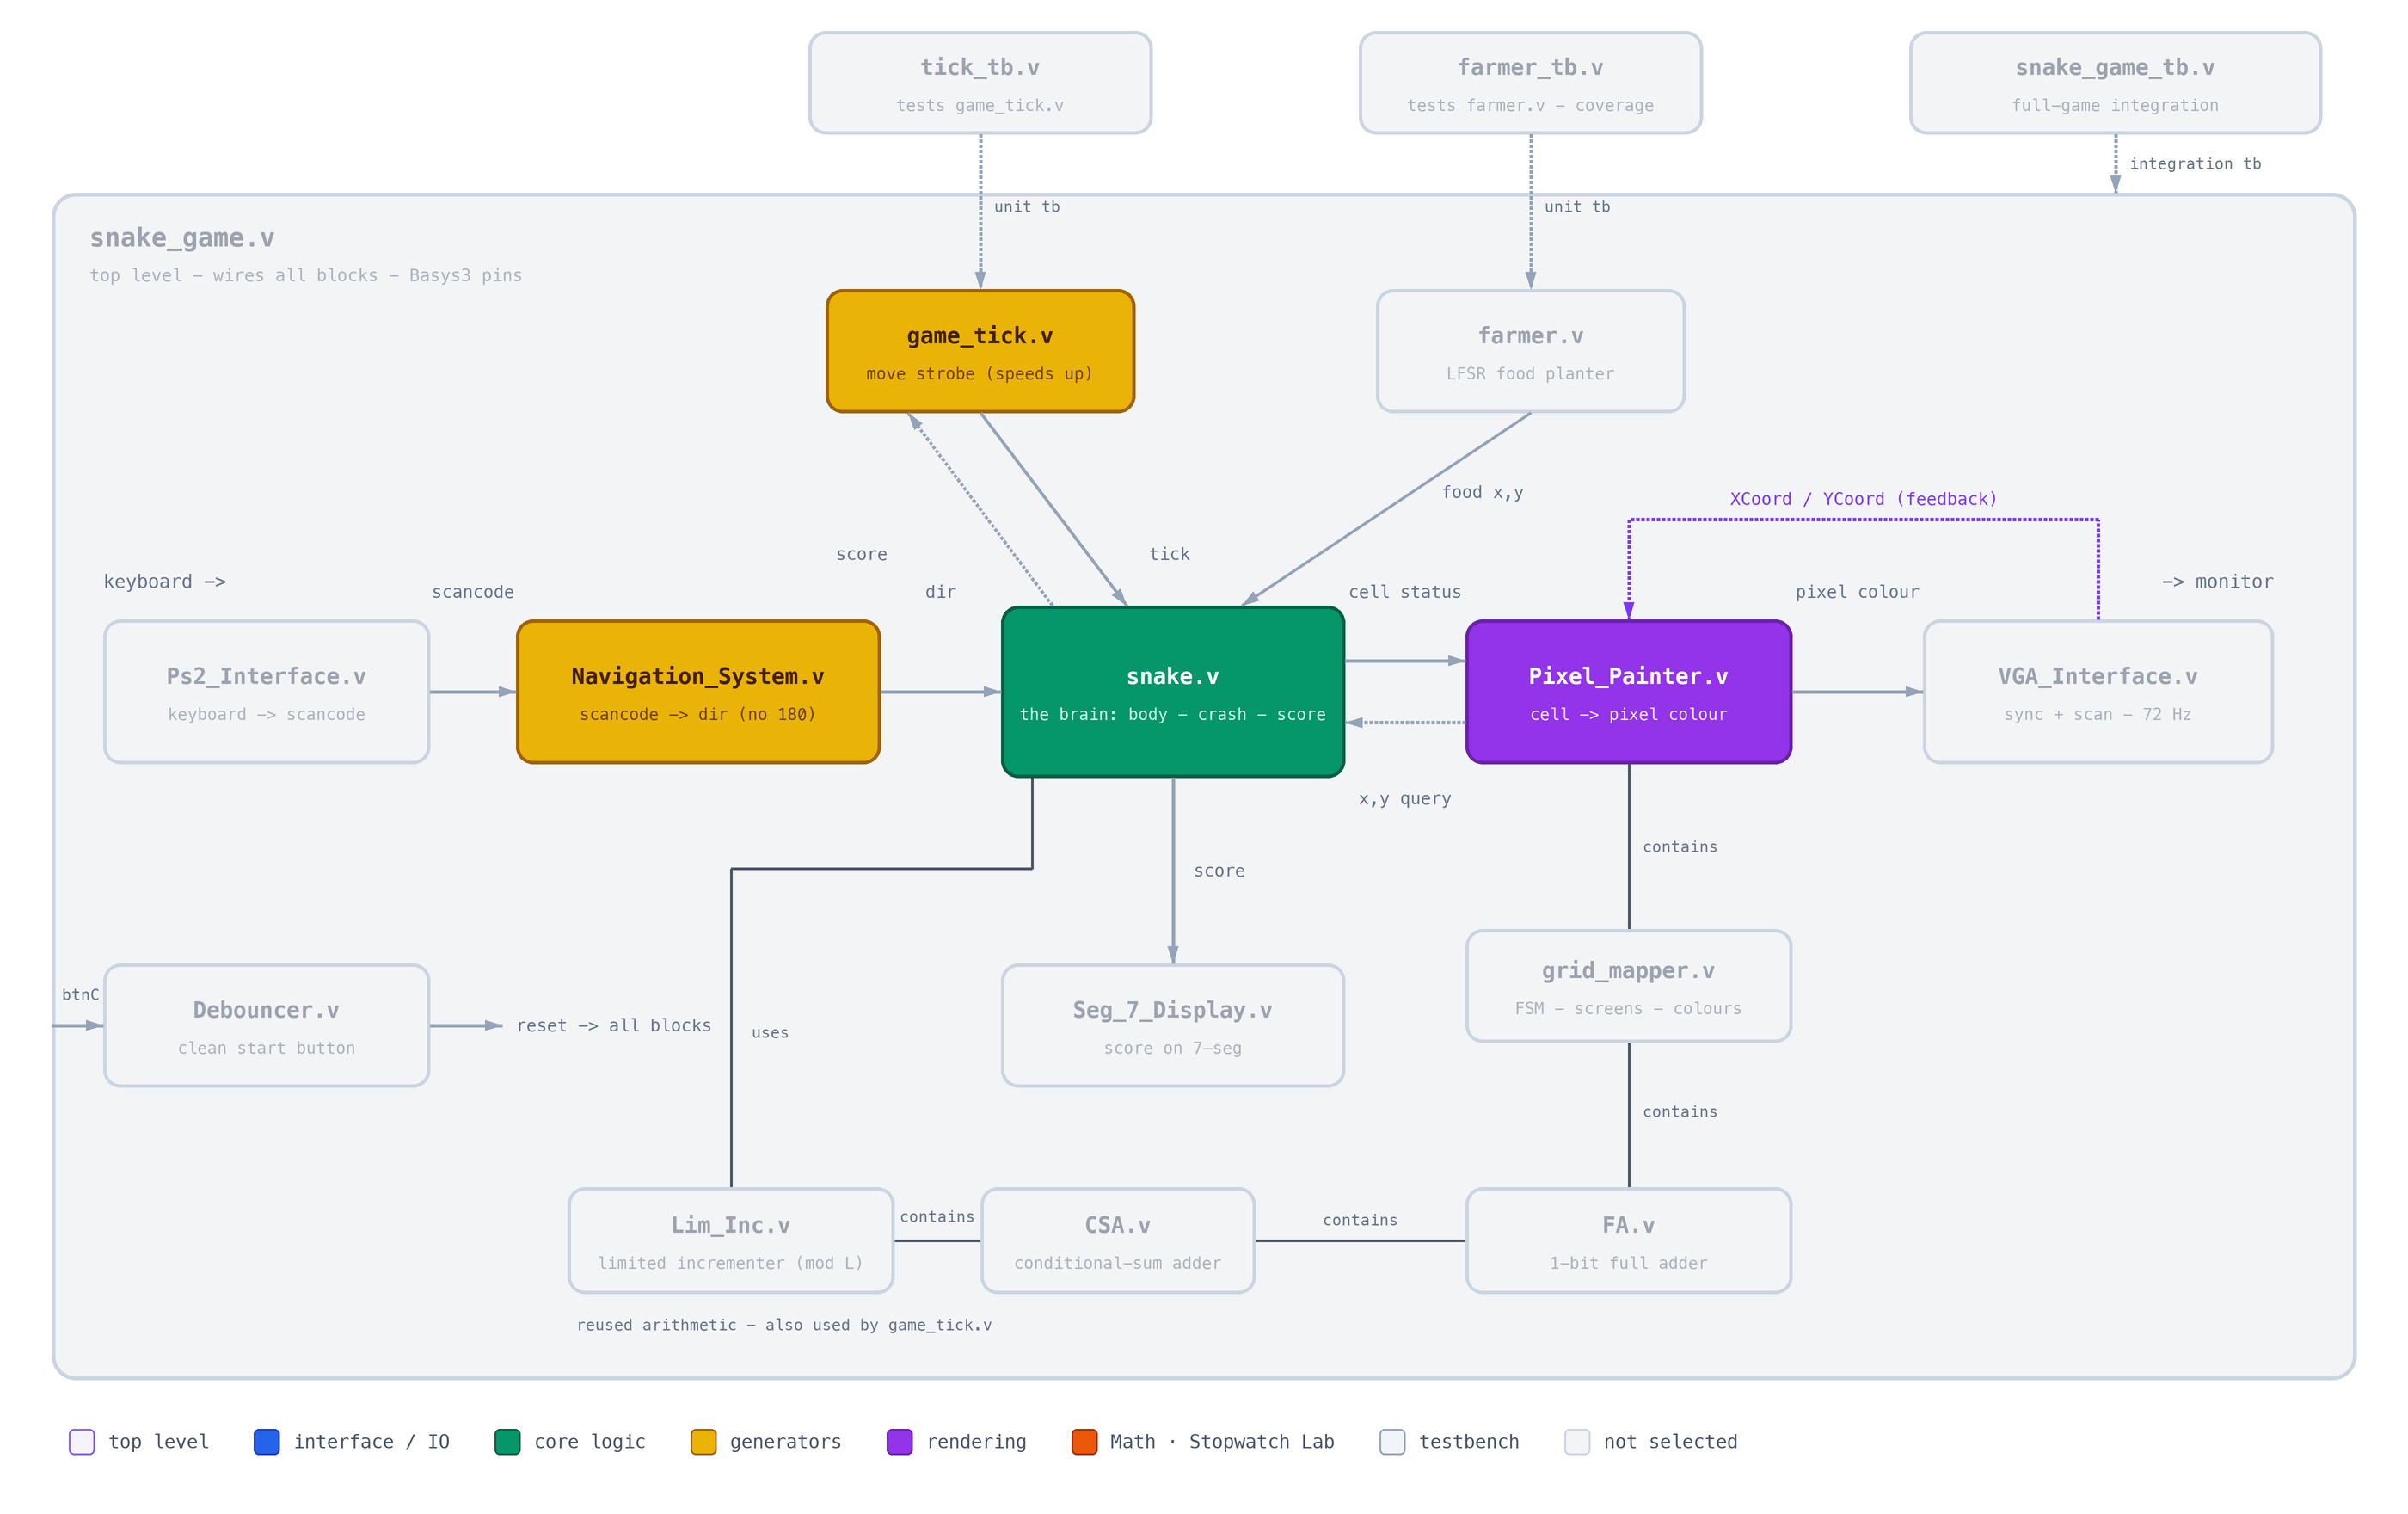
\includegraphics[width=\textwidth]{hierarchy_internal.png}
%   \caption{Internal logic modules highlighted.}
%   \label{fig:hier-internal}
% \end{figure}


% \textbf{Internal design.} The grid size is parameterised
% (\texttt{GRID\_X}$\,=100$, \texttt{GRID\_Y}$\,=75$) and forwarded to all
% parametric sub-modules, so a different grid granularity only requires
% changing these two parameters. The raw button is cleaned by
% \texttt{Debouncer} into the internal \texttt{reset}; the snake core is
% additionally held in reset until the welcome screen is dismissed
% (\texttt{reset | \textasciitilde start\_game}).

% \textbf{Verification -- \texttt{snake\_game\_tb.v}.} The integration
% testbench has no ports; it drives \texttt{clk}, \texttt{rst} and a
% behavioural PS/2 \emph{device} model that shifts real 11-bit frames
% (start bit, 8 data bits LSB-first, odd parity, stop bit) on
% \texttt{PS2Clk}/\texttt{PS2Data}, including the \texttt{F0} break codes.
% Because the real movement tick is $\approx$7\,Hz (14.3M clocks), the
% testbench forces a fast tick (one per 500 clocks) onto the internal
% \texttt{tick} net, then walks the game through a full scenario:
% start key $\rightarrow$ PLAY, steer up, steer left, run into the wall
% $\rightarrow$ GAME\_OVER, key $\rightarrow$ back to IDLE. One log line is
% printed per tick with the head position, length, direction, crash flag
% and FSM state.


\newpage
\subsection{\texttt{snake\_game\_tb.v} -- integration testbench}

\begin{itemize}
  \item \textbf{Scenario 1 - crash without eating} The snake drives
    straight into a wall without eating any food. The FSM transitions
    correctly (IDLE $\rightarrow$ PLAY $\rightarrow$ GAME\_OVER) and the
    length stays at 1 throughout.

    \begin{figure}[H]
  \centering
  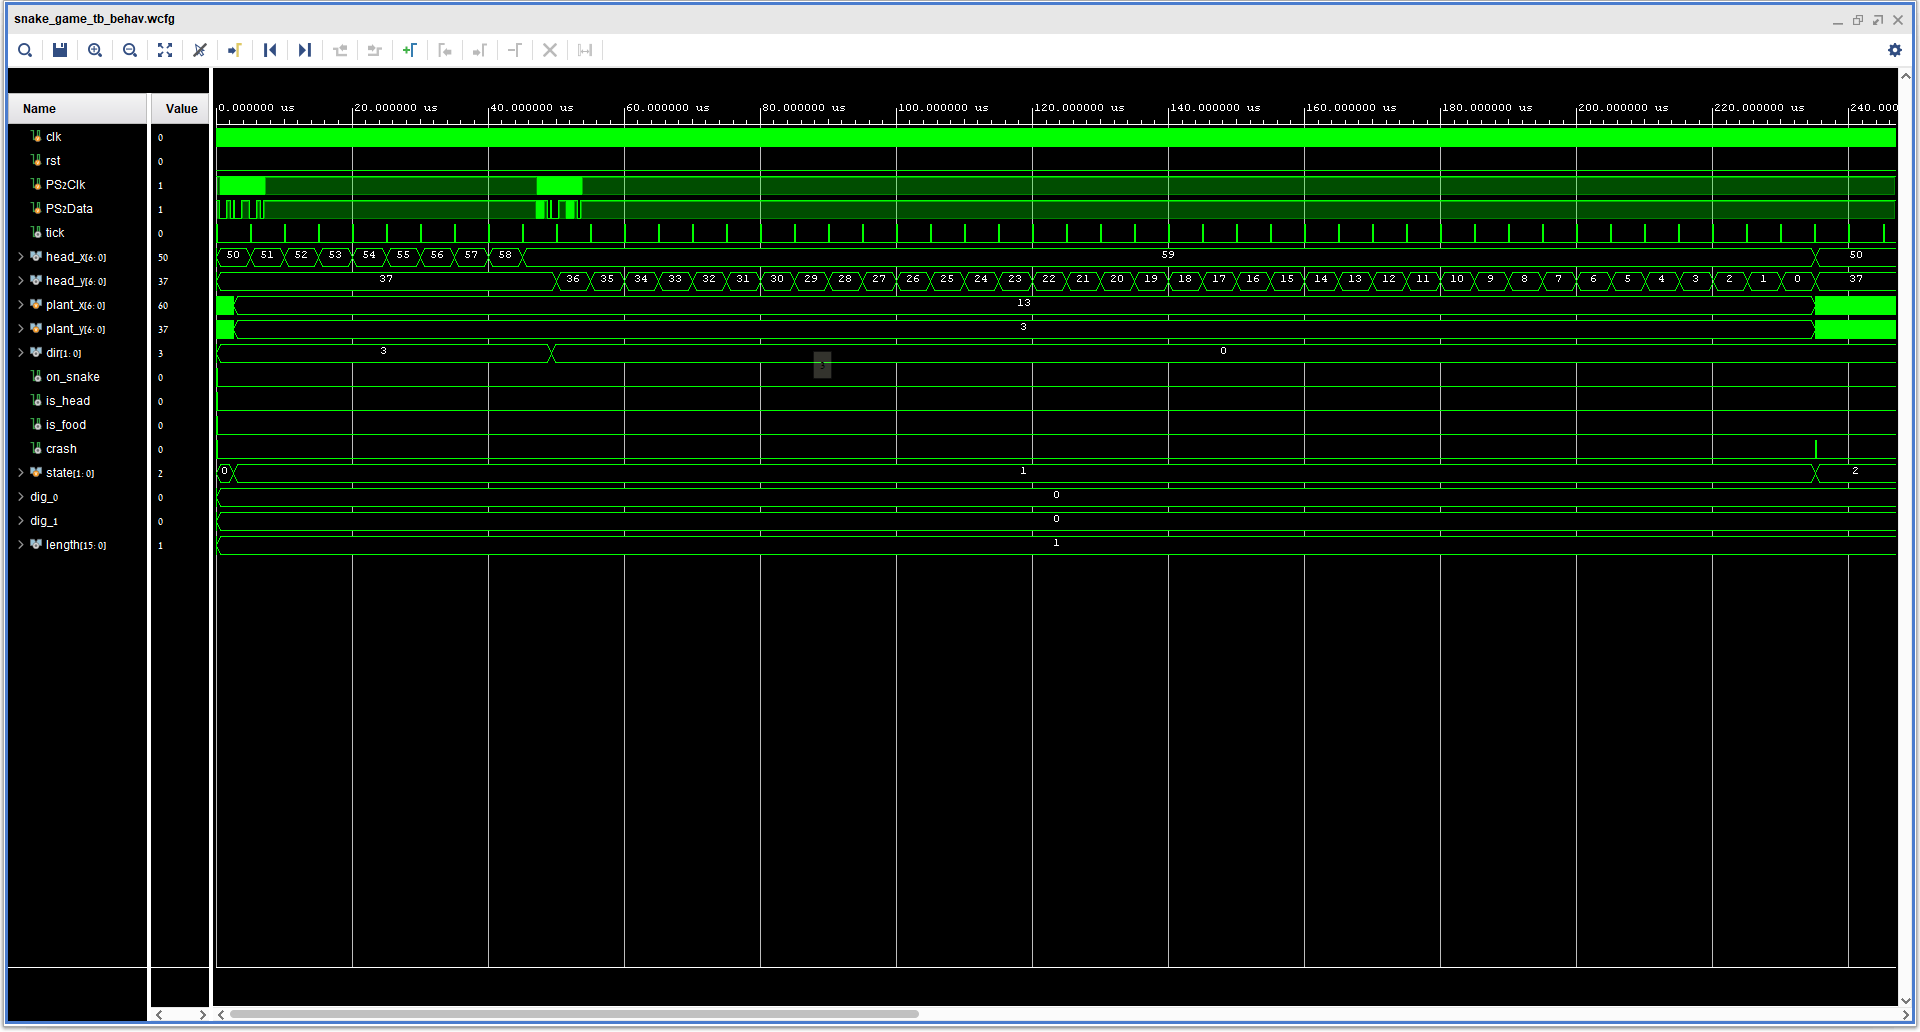
\includegraphics[width=\textwidth]{gm_tb_scenario_1.png}
  \caption{Scenario 1 - crash without eating}
  \label{fig:hier-io}
\end{figure}


  % \placeholderbox{5.2cm}{Annotated waveform of \texttt{snake\_game\_tb}
  %   Scenario 1: \texttt{keyPressed} pulses, \texttt{dir} changes,
  %   \texttt{tick} strobes, head coordinates advancing straight into a
  %   wall, \texttt{crash} rising, and the \texttt{state} transition to
  %   GAME\_OVER with \texttt{length} fixed at 1.}
  \item \textbf{Scenario 2 - eat then crash} The snake eats one food
    item, growing to length 2 and confirming that \texttt{snake.v}'s
    growth logic works, then crashes into a wall.


        \begin{figure}[H]
  \centering
  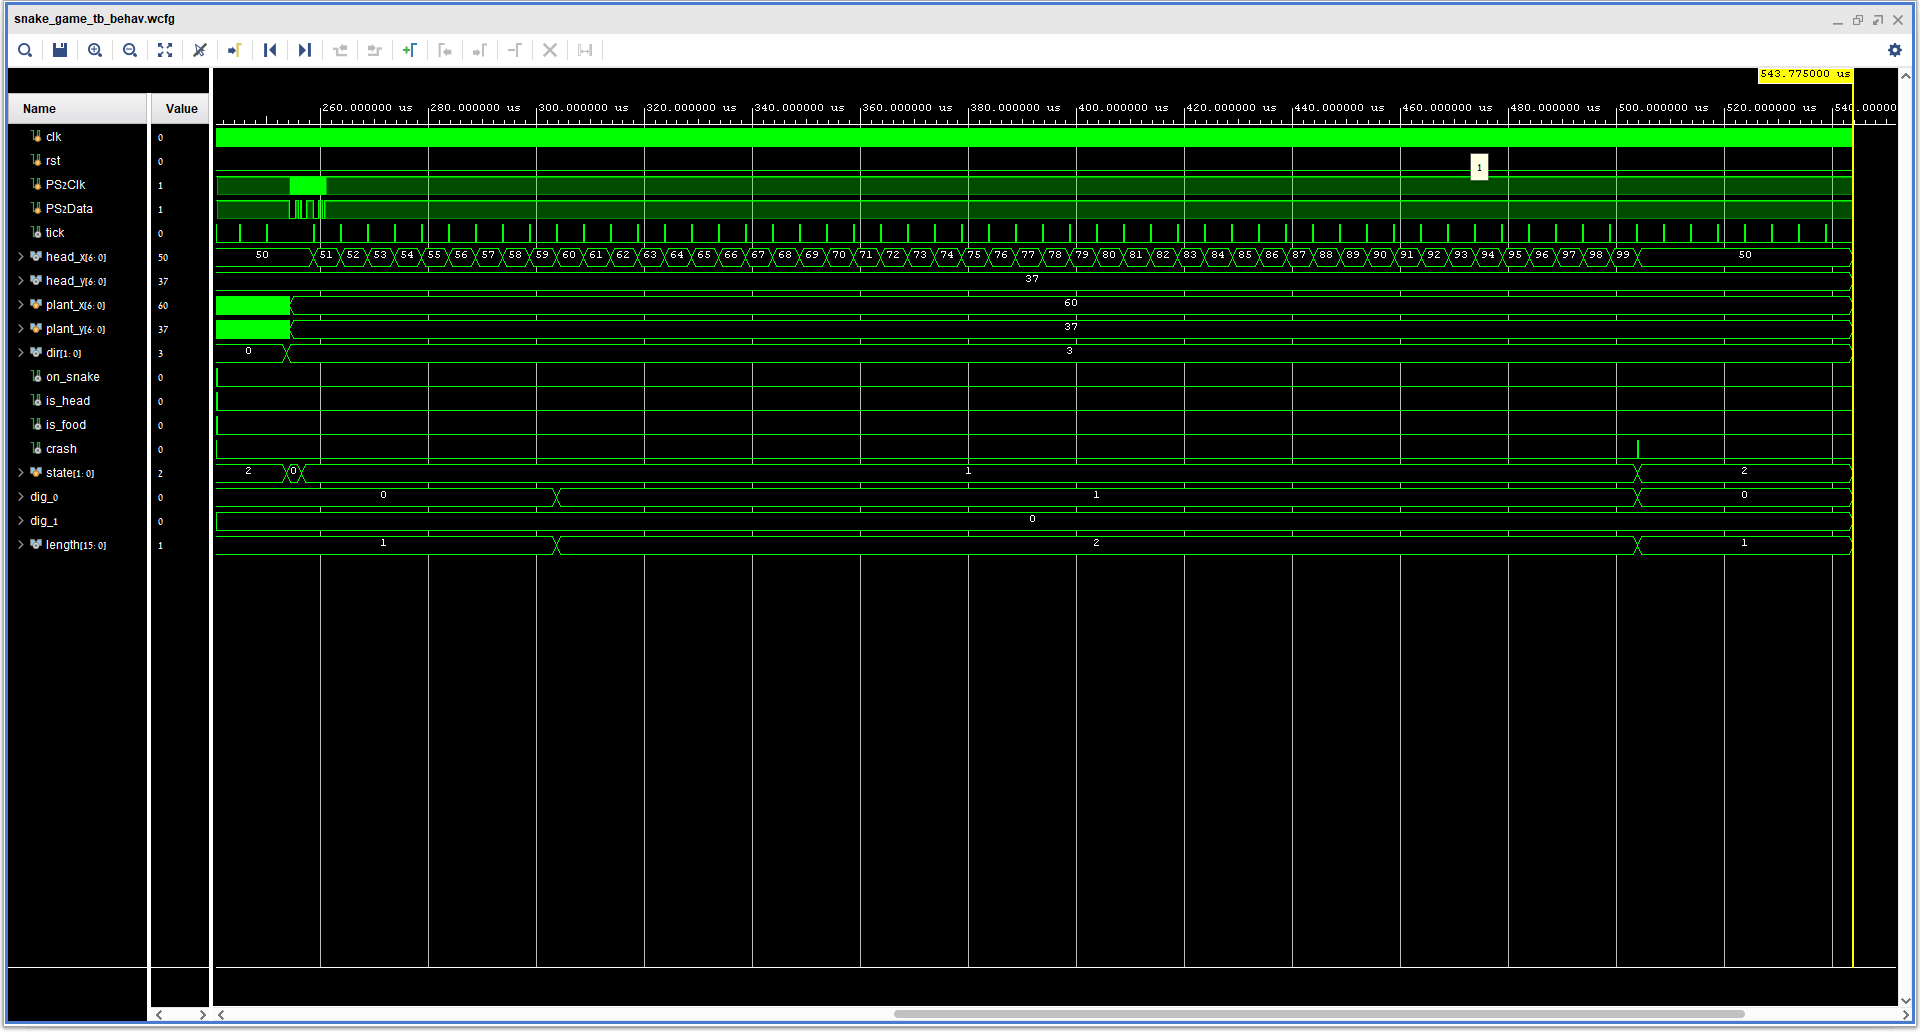
\includegraphics[width=\textwidth]{gm_tb_scenario_2.png}
  \caption{Scenario 2 - eat then crash}
  \label{fig:hier-io}
\end{figure}

    
  % \placeholderbox{5.2cm}{Annotated waveform of \texttt{snake\_game\_tb}
  %   Scenario 2: \texttt{keyPressed} pulses, \texttt{dir} changes,
  %   \texttt{tick} strobes, the food being eaten and \texttt{length}
  %   incrementing to 2, head coordinates advancing into a wall,
  %   \texttt{crash} rising, and the \texttt{state} transition to
  %   GAME\_OVER.}
\end{itemize}






% % =====================================================================
% \section{Input and Control Block}
% % =====================================================================
% This block turns the physical inputs (keyboard, push-button) into clean
% internal signals: \texttt{scancode}/\texttt{keyPressed}, the snake
% direction \texttt{dir}, and the global \texttt{reset}.

% % \begin{figure}[H]
% %   \centering
% %   
\includegraphics[width=\textwidth]{hierarchy_Ps2_Interface_Debouncer_Navigation_System.png}
% %   \caption{Input and control block highlighted.}
% % \end{figure}
% \placeholderbox{5cm}{Input and control block highlighted.}

% \subsection{\texttt{Ps2\_Interface.v}}
% \textbf{Purpose.} Receives PS/2 keyboard frames and outputs the make
% scancode with a single-clock \texttt{keyPressed} strobe.

% \begin{table}[H]
%   \centering\small
%   \caption{\texttt{Ps2\_Interface} interface.}
%   \begin{tabular}{lllp{0.45\textwidth}}
%     \toprule
%     \textbf{Port} & \textbf{Dir} & \textbf{Width} & \textbf{Description} \\
%     \midrule
%     \texttt{PS2Clk}  & in  & 1 & Keyboard-generated clock; data sampled on its falling edge. \\
%     \texttt{PS2Data} & in  & 1 & Serial data line. \\
%     \texttt{rstn}    & in  & 1 & Active-low reset. \\
%     \texttt{scancode} & out & 8 & Last accepted make code. \\
%     \texttt{keyPressed} & out & 1 & One-clock pulse per accepted key press. \\
%     \bottomrule
%   \end{tabular}
% \end{table}

% \textbf{Internal design.} A 22-bit shift register keeps the last two
% frames. Every 11 bits the current byte is examined: \texttt{E0}
% (extended) and \texttt{F0} (break prefix) are skipped, a byte following
% \texttt{F0} re-arms the receiver, and any other byte is latched as
% \texttt{scancode}. \texttt{keyPressed} fires only if odd parity checks
% out and the receiver is armed, so holding a key does not re-trigger
% until its break code arrives.

% \textbf{Verification.} Carried over from Lab 5, where it was verified
% with a dedicated testbench; in this lab it is exercised end-to-end by
% \texttt{snake\_game\_tb}, whose PS/2 device model sends full
% make/break sequences.

% \subsection{\texttt{Debouncer.v}}
% \textbf{Purpose.} Converts the bouncy centre push-button into a single
% one-clock reset pulse.

% \textbf{Internal design.} A saturating up/down hysteresis counter
% (parameter \texttt{COUNTER\_BITS}$\,=7$) counts towards all-ones while
% the input is high and back down while low; a pulse is emitted on the
% rising edge of the counter MSB. Genuinely parametric: the noise immunity
% grows exponentially with \texttt{COUNTER\_BITS}.

% \textbf{Verification.} Proven in earlier labs; exercised here through
% the integration testbench (see also Section~\ref{sec:problems} about its
% simulation-only X-propagation caveat).

% \subsection{\texttt{Navigation\_System.v}}
% \textbf{Purpose.} Maps scancodes to the 2-bit direction and blocks
% immediate reversals.

% \begin{table}[H]
%   \centering\small
%   \caption{Key mapping in \texttt{Navigation\_System}.}
%   \begin{tabular}{llll}
%     \toprule
%     \textbf{Key (numpad)} & \textbf{Scancode} & \textbf{Direction} & \textbf{Blocked while} \\
%     \midrule
%     4 & \texttt{0x6B} & LEFT  & RIGHT \\
%     6 & \texttt{0x74} & RIGHT & LEFT  \\
%     8 & \texttt{0x75} & UP    & DOWN  \\
%     5 & \texttt{0x73} & DOWN  & UP    \\
%     \bottomrule
%   \end{tabular}
% \end{table}

% \textbf{Internal design.} A clocked \texttt{case} on \texttt{scancode},
% qualified by \texttt{keyPressed}. Each assignment is guarded by
% ``\texttt{if (dir != opposite)}'', which implements requirement 3b
% directly in hardware. On reset the direction defaults to RIGHT. Any
% other key leaves \texttt{dir} unchanged (but still wakes the game from
% the welcome screen through \texttt{keyPressed}).

% \textbf{Verification.} Exercised by \texttt{snake\_game\_tb}: the
% scenario steers UP then LEFT and the log shows the head turning
% accordingly; a reversal attempt is visible as an ignored key.

% =====================================================================
\section{Internal Game Logic}
% =====================================================================
\begin{figure}[H]
  \centering
  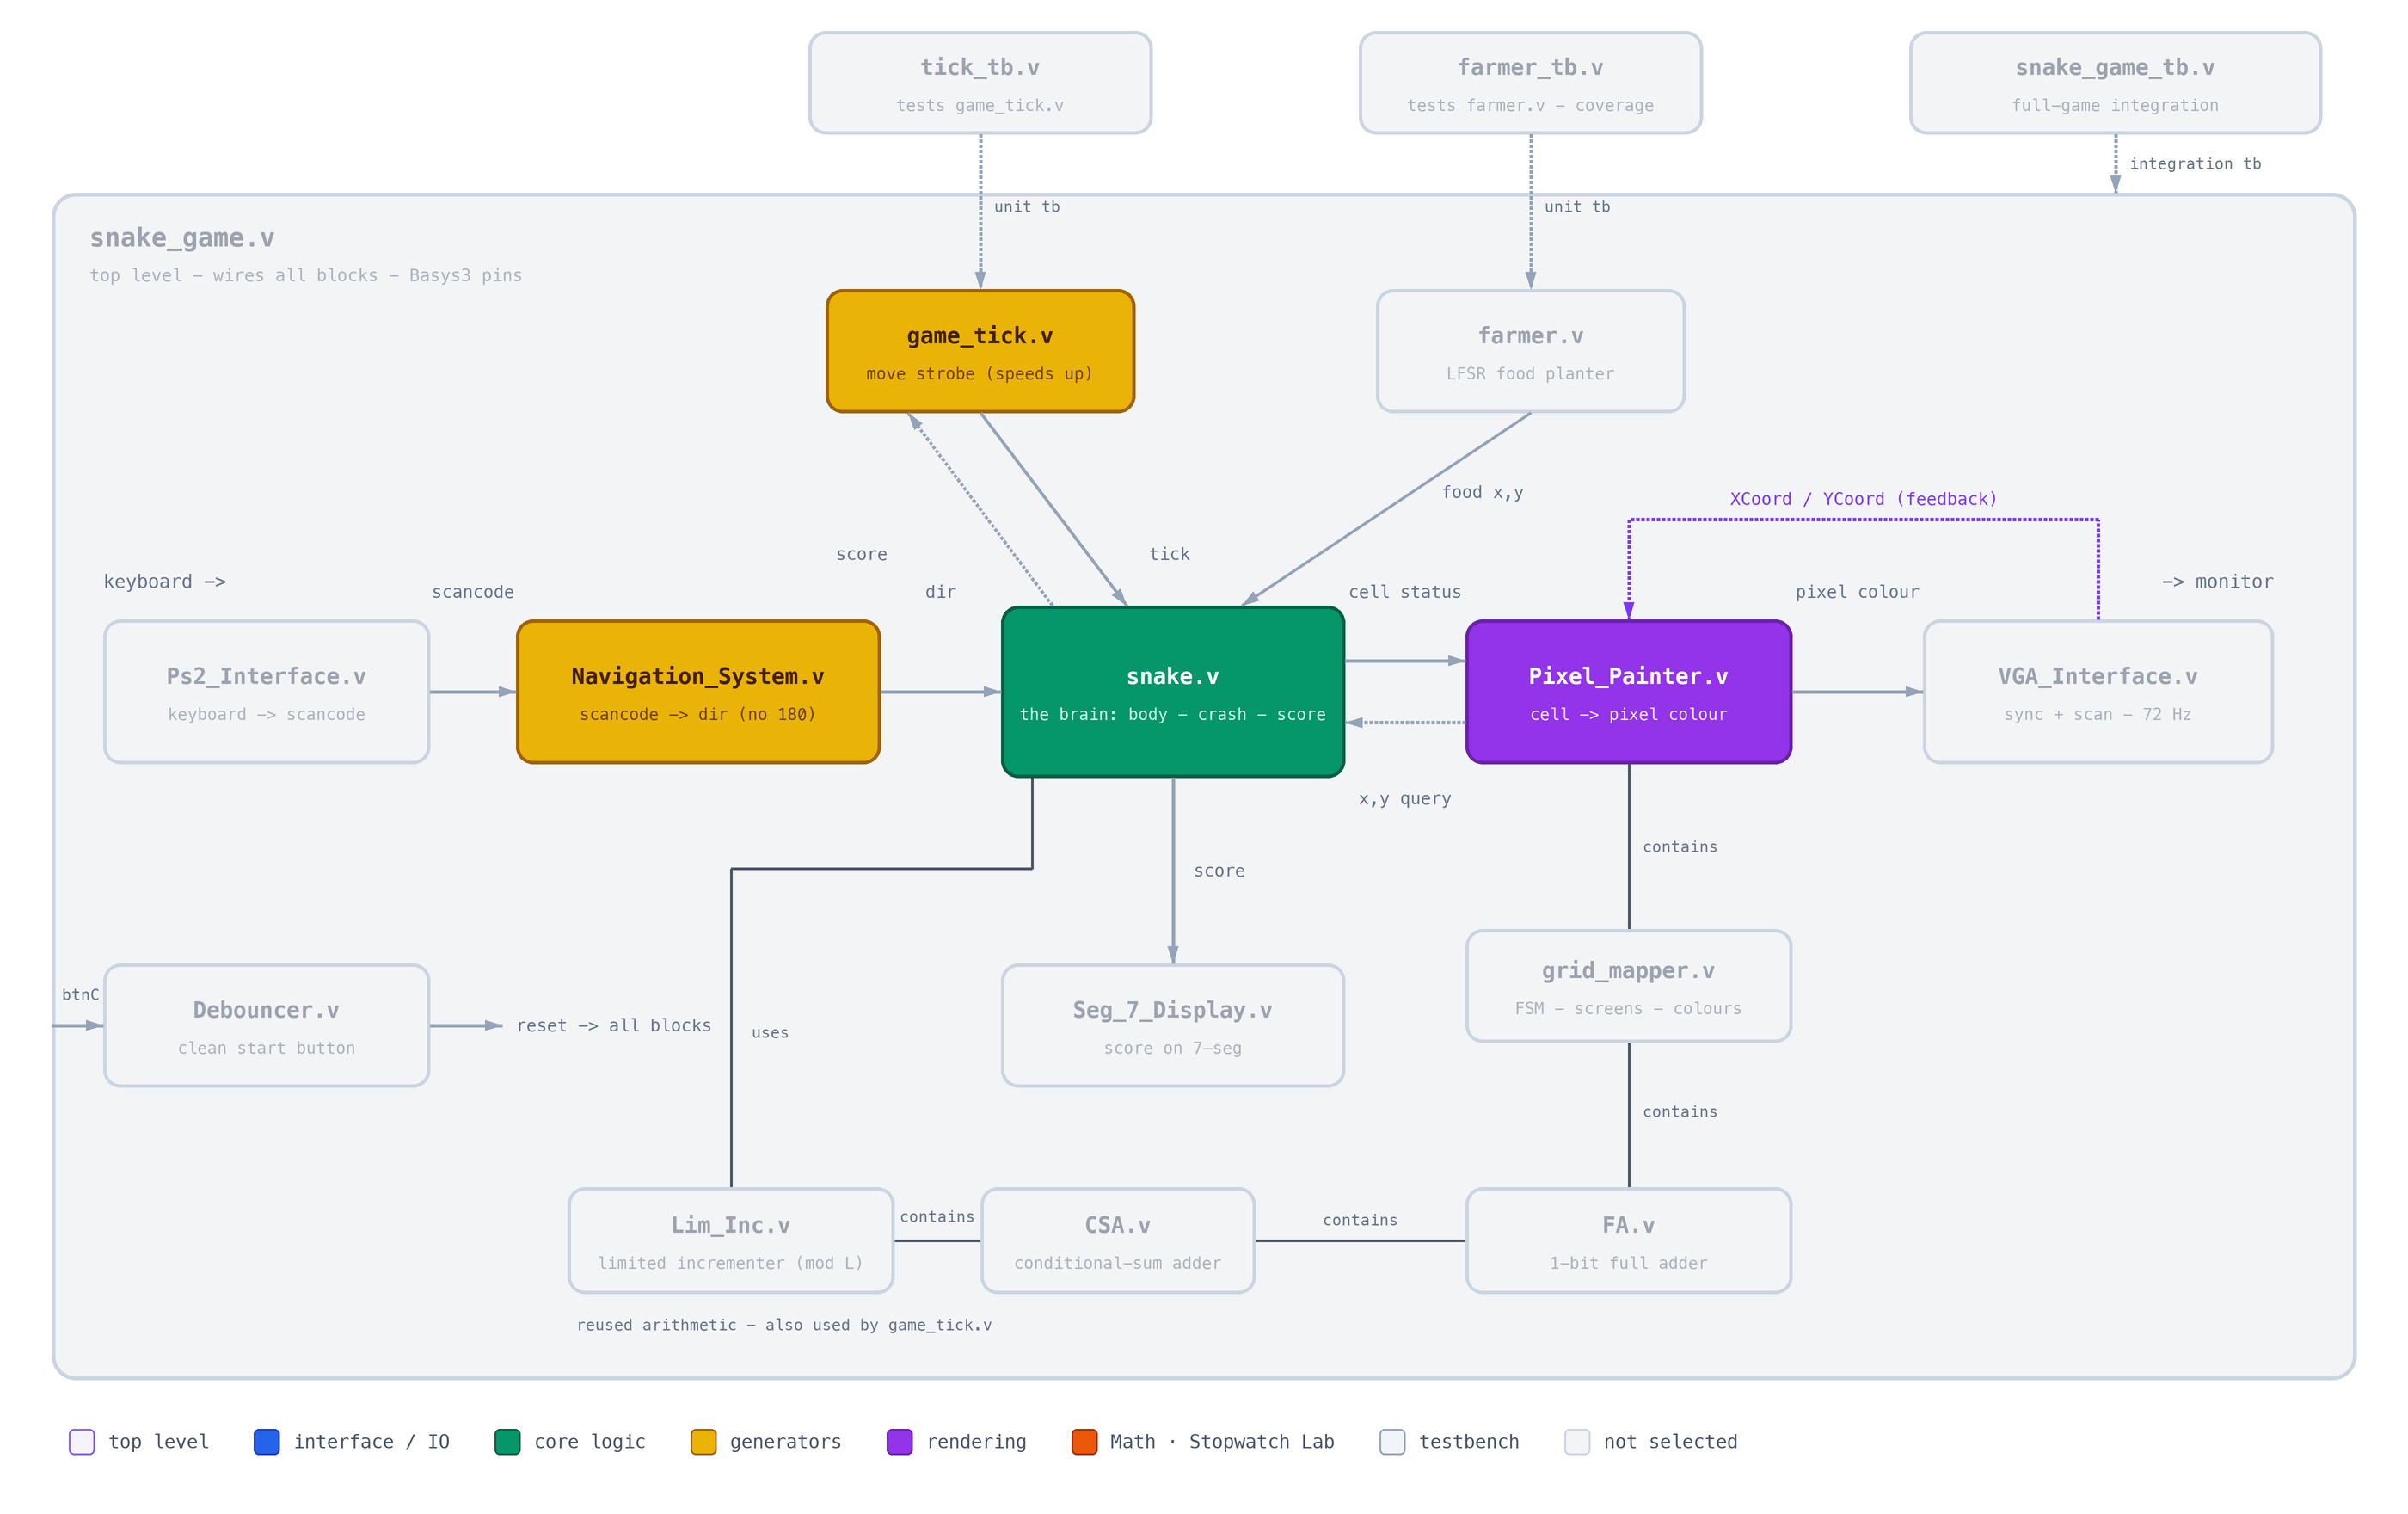
\includegraphics[width=\textwidth]{hierarchy_internal.png}
  \caption{Internal logic modules highlighted.}
  \label{fig:hier-internal}
\end{figure}
% \placeholderbox{5cm}{Game-logic block highlighted: the snake core, its food
% generator and the food-coverage testbench.}

\subsection{\texttt{snake.v} - the game core}
\textbf{Purpose.} Owns the snake body, movement, growth, collision
detection and score.

\begin{table}[H]
  \centering\small
  \caption{\texttt{Snake} interface (parameters \texttt{GRID\_X}, \texttt{GRID\_Y}).}
  \begin{tabular}{lllp{0.42\textwidth}}
    \toprule
    \textbf{Port} & \textbf{Dir} & \textbf{Width} & \textbf{Description} \\
    \midrule
    \texttt{clk}, \texttt{reset} & in & 1 & Clock and synchronous reset. \\
    \texttt{tick} & in & 1 & Movement strobe from \texttt{Game\_Tick}. \\
    \texttt{dir}  & in & 2 & Direction from \texttt{Navigation\_System}. \\
    \texttt{keyPressed} & in & 1 & Entropy for the food LFSR. \\
    \texttt{x}, \texttt{y} & in & 7/7 & Cell queried by the renderer. \\
    \texttt{on\_snake}, \texttt{is\_head}, \texttt{is\_food} & out & 1 &
      Answers to the query: body / head / food at $(x,y)$. \\
    \texttt{crash} & out & 1 & Latched game-over flag. \\
    \texttt{score} & out & 16 & Current score (= snake length). \\
    \bottomrule
  \end{tabular}
\end{table}

\textbf{Internal design.} The body is stored as two coordinate register
arrays \texttt{body\_x/body\_y[0..63]} (\texttt{MAX\_LEN}$=64$) with the
head at index 0. Movement is a shift: on every tick each element copies
its predecessor and the head takes the freshly computed next position.
Combinational logic computes the next head from \texttt{dir}, and a
64-way comparison loop checks whether the next head lands on the body
(self collision) or the query cell lies on the body (render query). To
relax timing, the next-head, self-hit and eat signals are registered one
clock before being consumed (\texttt{next\_x\_r}, \texttt{hit\_self\_r},
\texttt{is\_eaten\_r}, \texttt{tick\_d}). A crash is latched when the
next head leaves the grid or hits the body; growth happens when the next
head equals the food cell. The food position proposed by \texttt{farmer}
is latched into \texttt{plant\_x/plant\_y} only when the food is eaten
(or at reset), so the food stays put between meals.

\textbf{Verification.} Exercised in full by \texttt{snake\_game\_tb}
(movement, steering, growth, wall crash, restart); the per-tick log
prints head position and length so the shift behaviour is directly
observable.

\subsubsection{\texttt{farmer.v} - food generator}

\begin{figure}[H]
  \centering
  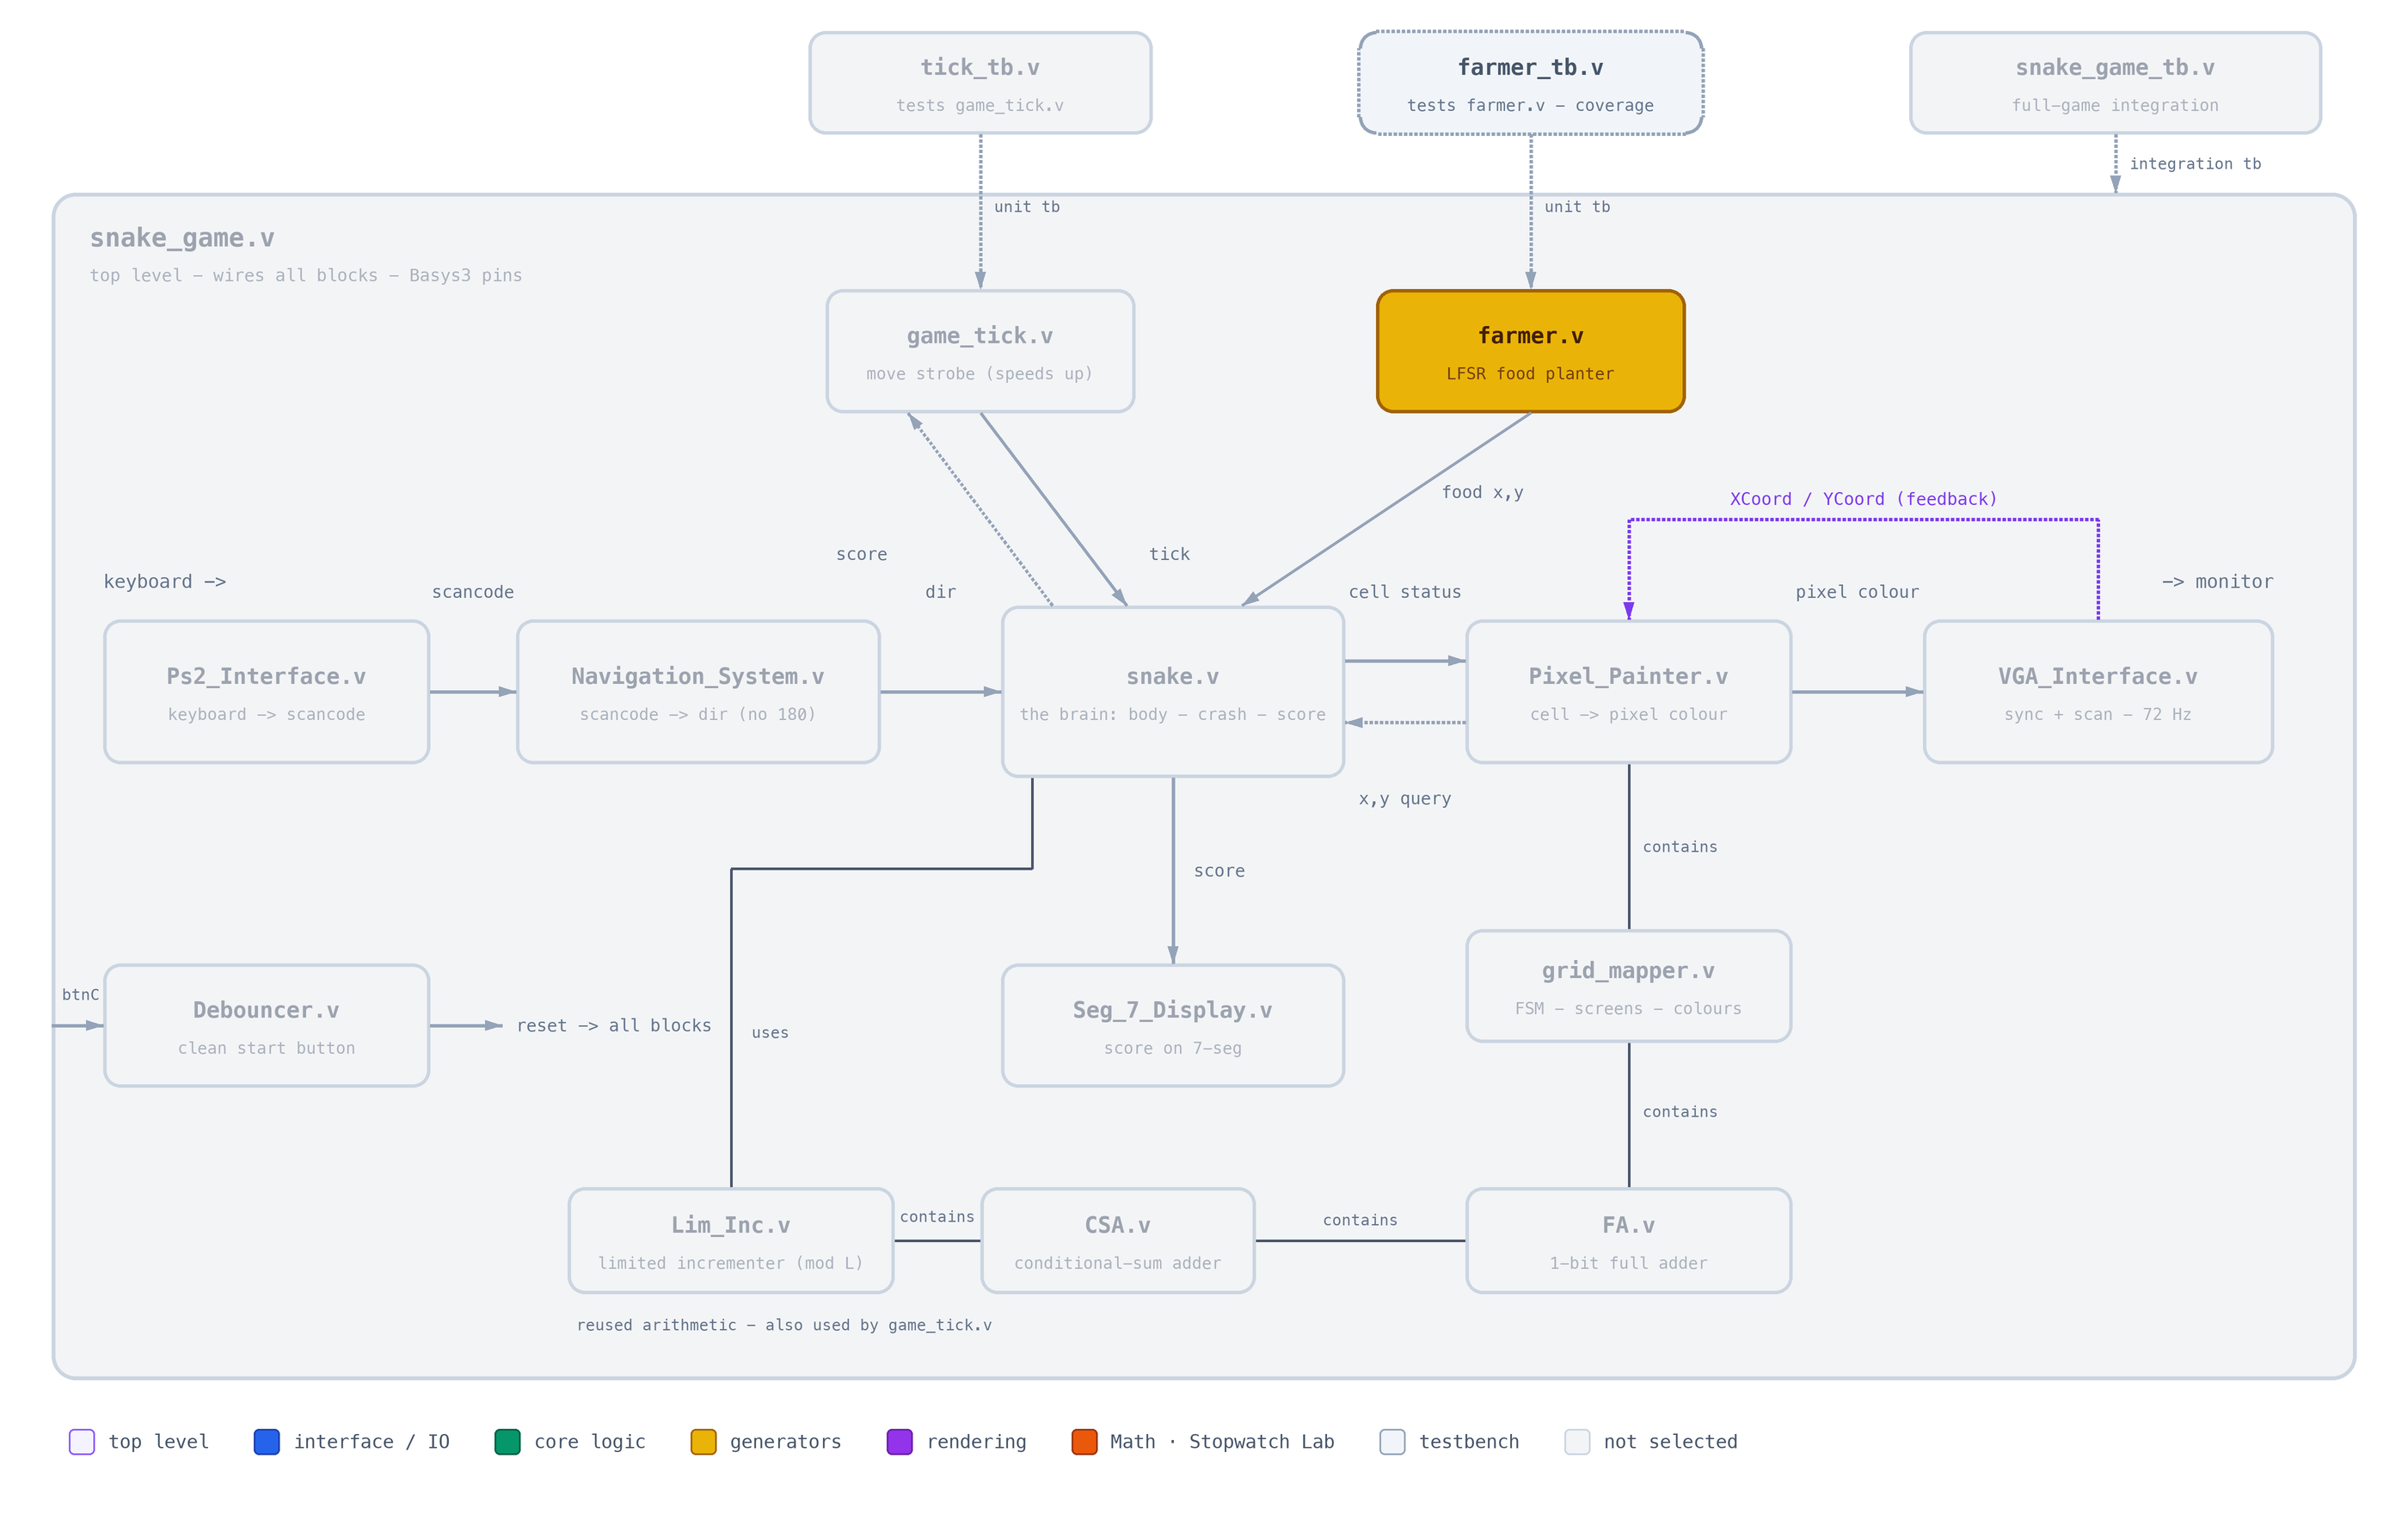
\includegraphics[width=0.8\textwidth]{hierarchy_farmer_farmer_tb.png}
  % \caption{Food-placement coverage recorded by \texttt{farmer\_tb}
  % ($15{,}000$ samples on the $100\times75$ grid; green = proposed at
  % least once, dark = never proposed).}
  \label{fig:farmer}
\end{figure}

\textbf{Purpose} This module serves as a pseudo-random food coordinates generator for the food position on the board (\texttt{food\_x}, \texttt{food\_y}). \\
\textbf{Internal design} It holds a 16-bit shift register 
that shifts left every clock (\texttt{100 MHz clk}), and the LSB becomes the \texttt{Xor} of the \texttt{lfsr[15], lfsr[13], lfsr[12], lfsr[10], keyPressed}
the Farmer generates output that looks random but it raility is fully deterministic so we choose to make the shift every clock and use the \texttt{keyPressed} as an entropy source to make the output less predictable. The food coordinates are computed as follows:
$\texttt{food\_x} = \texttt{lfsr}[6{:}0] \bmod \texttt{GRID\_X}$ and
$\texttt{food\_y} = \texttt{lfsr}[13{:}7] \bmod \texttt{GRID\_Y}$.


\textbf{Verification} The 
testbench clocks the shift register $15{,}000$ times ($\approx 2$ proposals per
grid cell), toggles \texttt{keyPressed} randomly ($\approx 1\%$ of
clocks) and records every proposed coordinate. 

\begin{figure}[H]
  \centering
  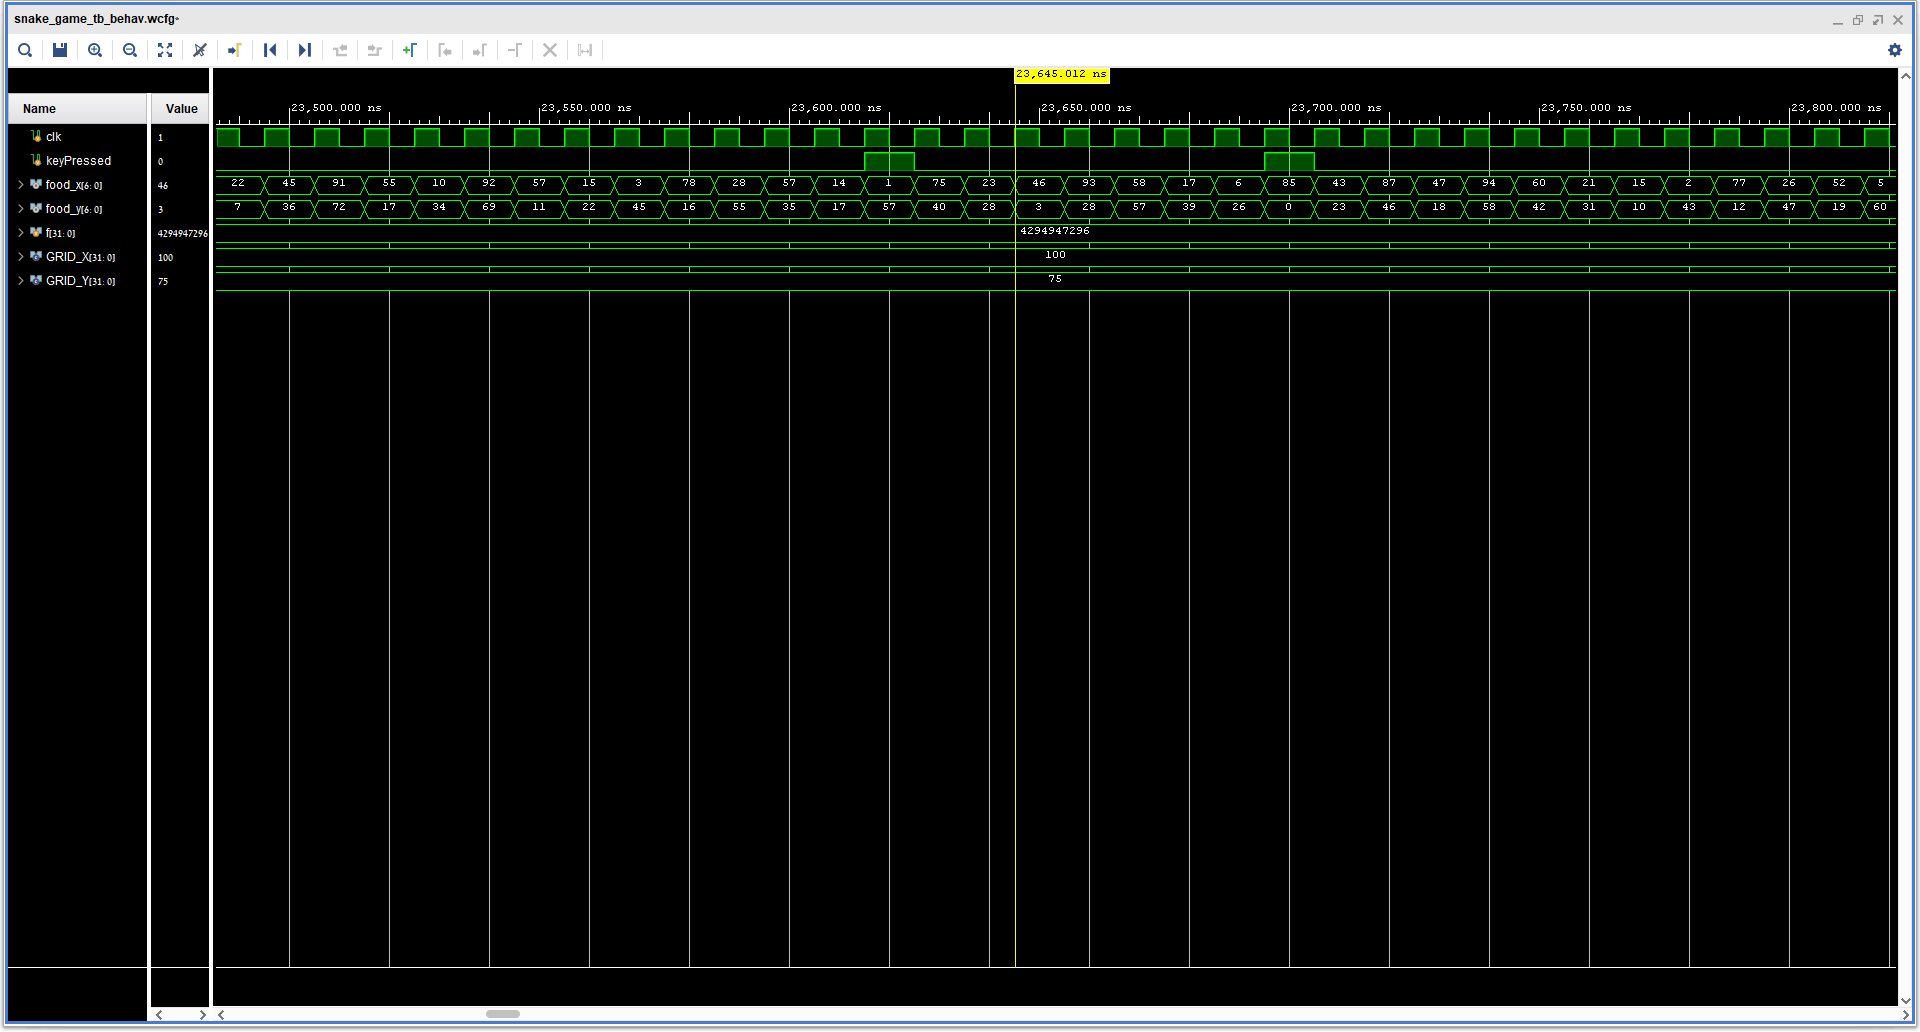
\includegraphics[width=0.8\textwidth]{farmer_wavefrom.png}
  \caption{Food-placement coverage recorded by \texttt{farmer\_tb}
  ($15{,}000$ samples on the $100\times75$ grid; green = proposed at
  least once, dark = never proposed).}
  \label{fig:coverage}
\end{figure}

The map also makes the \emph{modulo bias} of the generator visible: as
\texttt{food\_x} is a 7-bit value (0--127) reduced mod 100, columns
0--27 are proposed twice as often -- the denser left band in the figure;
likewise rows 0--52 for \texttt{food\_y} (mod 75). Every cell of the
grid is reachable, and the bias is invisible during play, so this was
accepted as a good trade-off for such a cheap generator.


\textbf{Coverage} 
Figure~\ref{fig:coverage}
shows the resulting coverage of the $100\times75$ grid: green cells were
proposed at least once, dark cells never(we have achived $\approx 81\%$  coverage) so we can confidently say that the farmer is good enogh to generate food coordinates.

\begin{figure}[H]
  \centering
  
\includegraphics[width=0.8\textwidth]{food_coverage.png}
  \caption{Food-placement coverage recorded by \texttt{farmer\_tb}
  ($15{,}000$ samples on the $100\times75$ grid; green = proposed at
  least once, dark = never proposed).}
  \label{fig:coverage}
\end{figure}

% =====================================================================
% \section{Timing Block}
% =====================================================================


\subsection{\texttt{game\_tick.v}}
\textbf{Purpose.} Generates the movement strobe and implements the
difficulty ramp: the higher the score, the faster the snake.


\begin{figure}[H]
  \centering
  
\includegraphics[width=\textwidth]{hierarchy_game_tick_tick_tb.png}
  \caption{Timing block highlighted.}
\end{figure}



\textbf{Internal design.} A counter compares against a programmable
period \texttt{tick\_speed} and emits a one-clock \texttt{tick} pulse on
wrap-around. The period starts at the parameter
\texttt{TICK\_MAX} ($14{,}285{,}714$ clocks $= 7$\,Hz at 100\,MHz) and
decreases linearly with the score:
\[
  \texttt{tick\_speed} = \texttt{TICK\_MAX} - \texttt{score}\cdot 2^{18},
\]
clamped after 54 steps so the period never underflows. The module is
fully parametric in \texttt{TICK\_MAX} (the testbench and top level both
instantiate it explicitly with their own value).

\begin{table}[H]
  \centering\small
  \caption{Tick rate vs.\ score (at 100\,MHz, \texttt{TICK\_MAX}$=14{,}285{,}714$).}
  \begin{tabular}{lccccc}
    \toprule
    \textbf{Score} & 1 & 10 & 20 & 30 & 40 \\
    \midrule
    \textbf{Tick rate} & 7.1\,Hz & 8.6\,Hz & 11.1\,Hz & 15.6\,Hz & 26.3\,Hz \\
    \bottomrule
  \end{tabular}
\end{table}

\textbf{Verification -- \texttt{tick\_tb.v}.} The unit testbench sweeps
the score through $0, 10, 50, 60, 64, 80$ (crossing the clamp) and
exposes the internal period plus a derived frequency probe
(\texttt{hz = 100\,MHz / tick\_speed}) so the ramp and the clamping are
directly visible in the waveform.

\placeholderbox{4.6cm}{Annotated waveform of \texttt{tick\_tb}: arrows on
the shrinking distance between \texttt{tick} pulses as \texttt{score}
steps up, and on \texttt{tick\_speed} saturating once the clamp
(score $\geq 54$) is reached.}

% =====================================================================
\subsection{Rendering Block}

\begin{figure}[H]
  \centering
  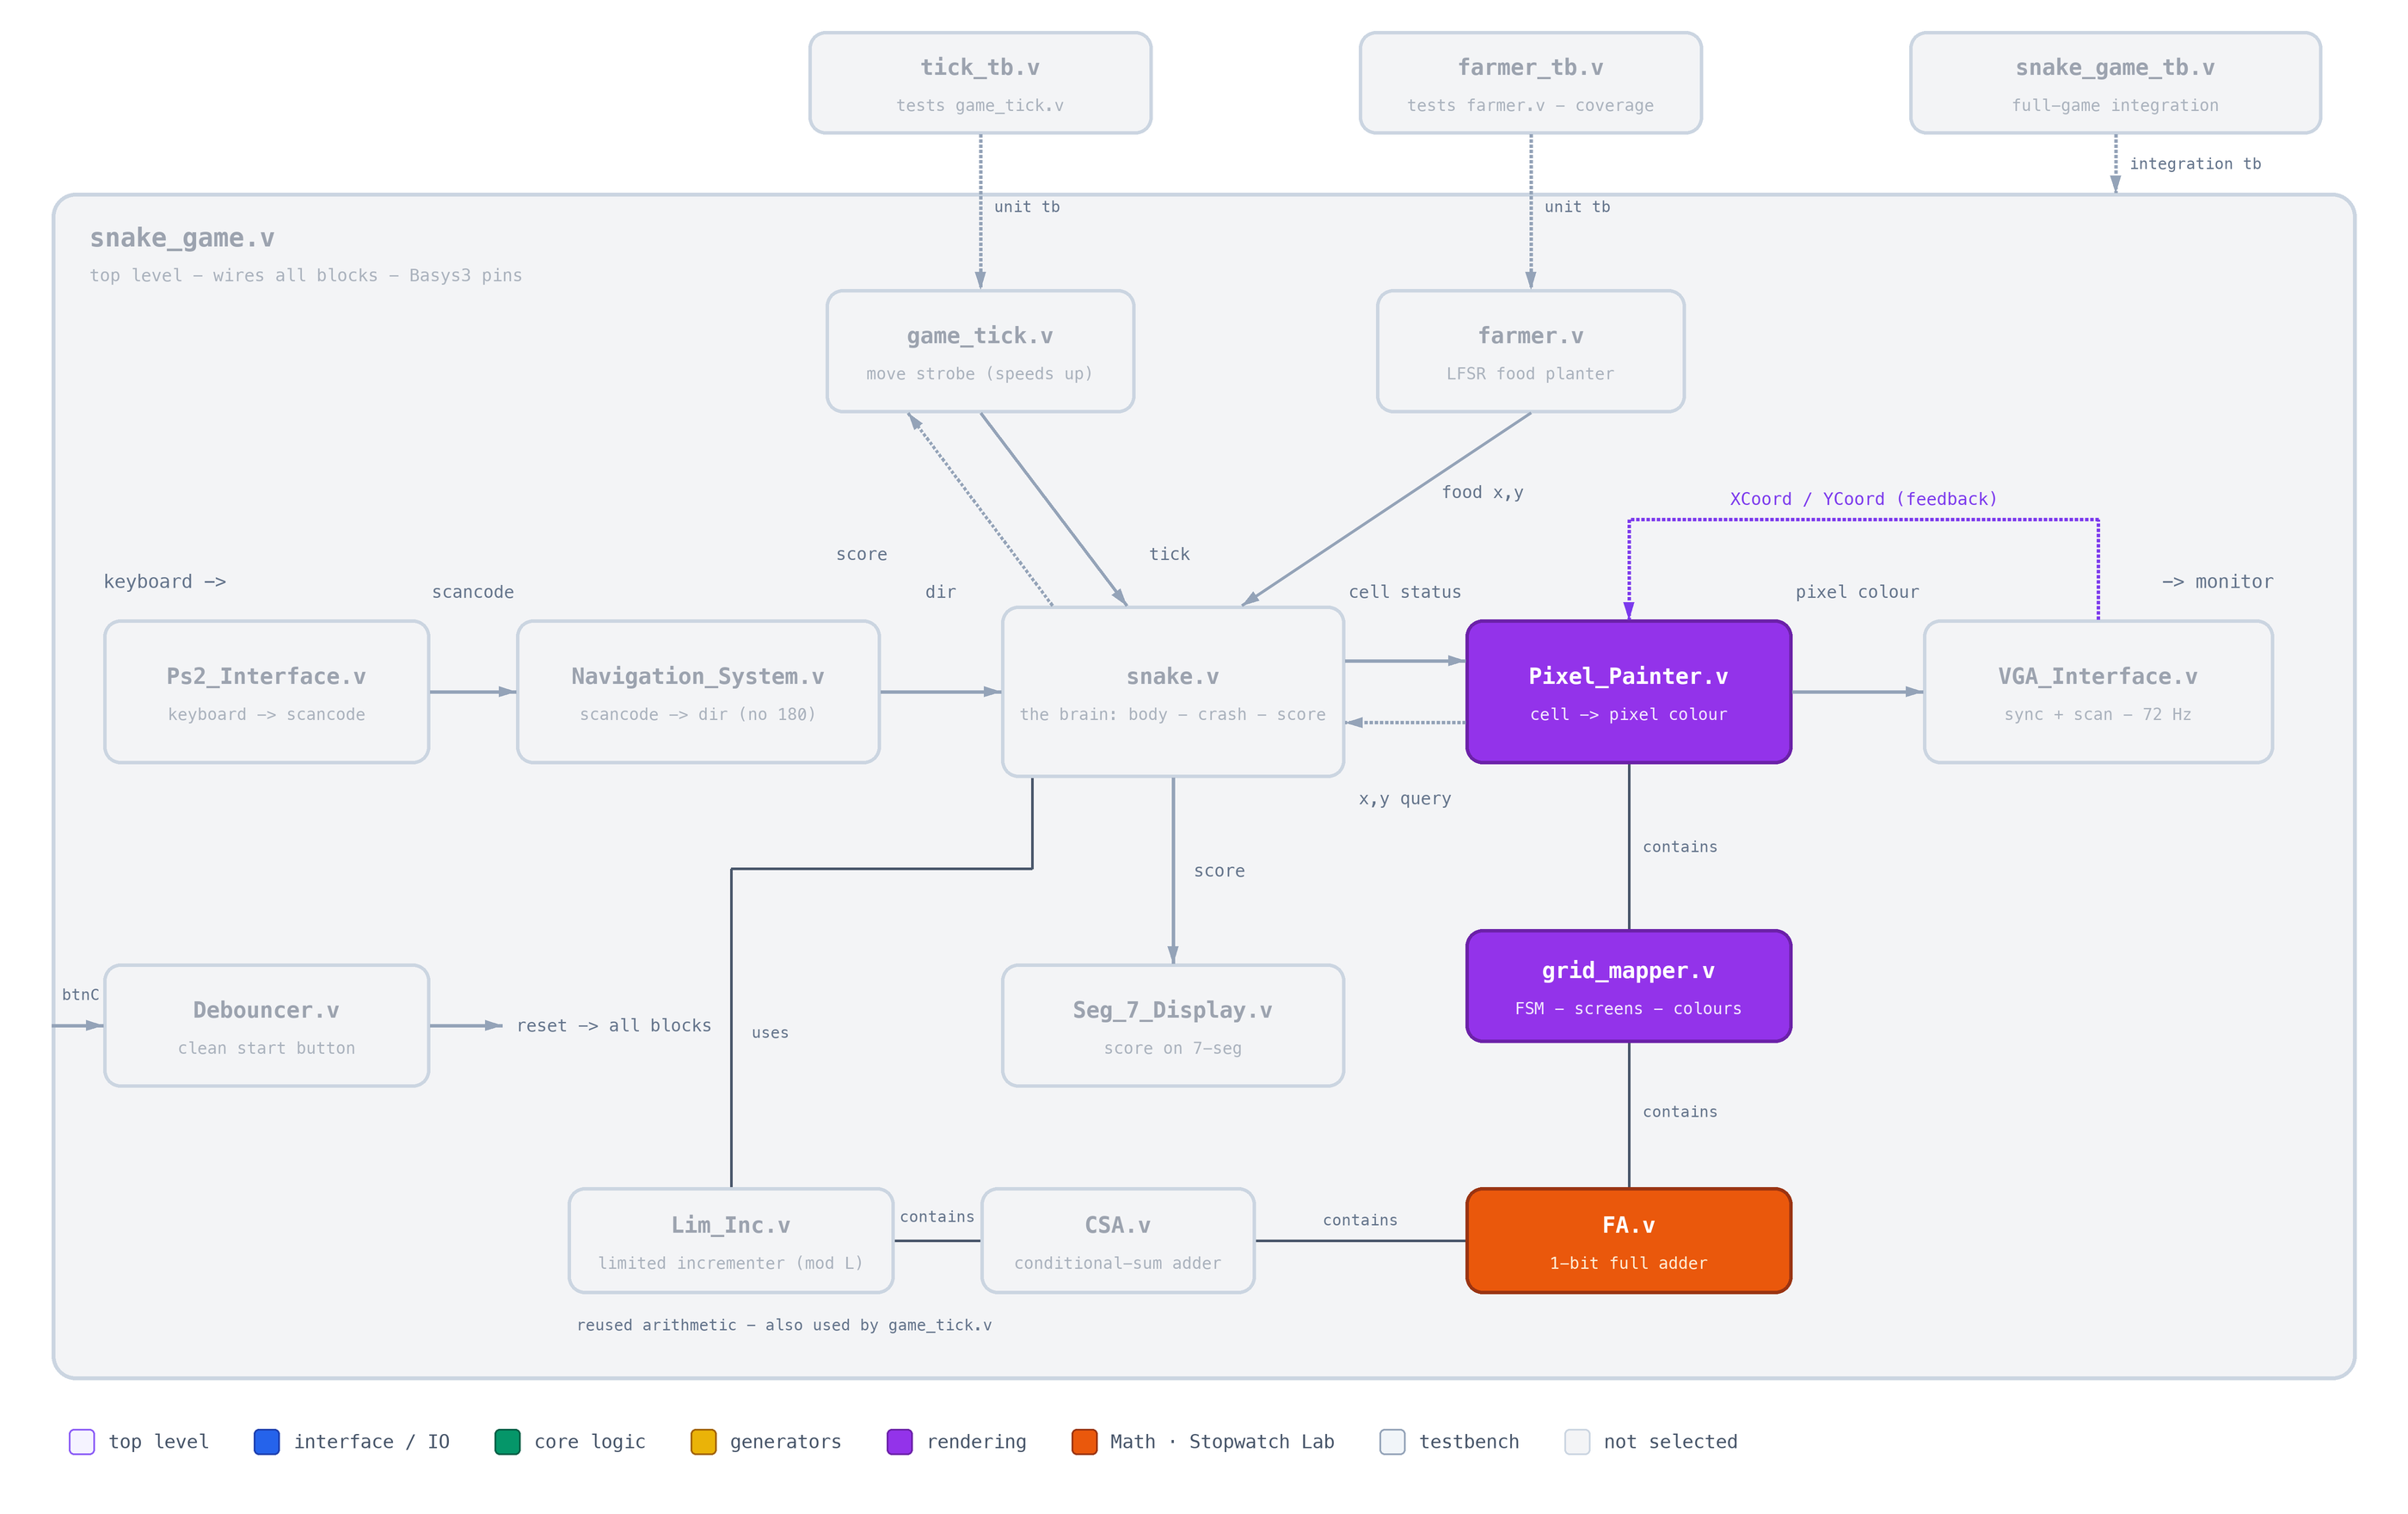
\includegraphics[width=\textwidth]{hierarchy_screen_render.png}
  \caption{Rendering block highlighted}
\end{figure}
% =====================================================================

\placeholderbox{5cm}{Rendering block highlighted.}

\subsubsection{\texttt{Pixel\_Painter.v}}
\textbf{Purpose.} Bridges between the pixel domain (VGA scan
coordinates) and the cell domain (game grid), and composes the final
pixel color.

\textbf{Internal design.} The scan position is divided by 8
(\texttt{XCoord >> 3}) to obtain the queried grid cell $(x,y)$, and by 4
to obtain the $200\times150$ bitmap coordinates used by the splash
screens. The cell color returned by \texttt{GridMapper} is overlaid
with black 1-pixel grid lines (every 8th row/column) while the game is
in PLAY; \texttt{start\_game} (i.e.\ ``the game is on the PLAY screen'')
is exported to the top level, where it releases the snake core from
reset.

\subsubsection{\texttt{grid\_mapper.v}}
\textbf{Purpose.} The screen FSM and color oracle: decides \emph{what
is shown} for every cell in each game phase.

\textbf{Internal design.} A three-state FSM -- IDLE (welcome screen),
PLAY, GAME\_OVER -- advances on \texttt{keyPressed} and \texttt{crash}.
Two $200\times150$ monochrome bitmaps are preloaded with
\texttt{\$readmemb} into block RAM: the welcome splash and the skull
``YOU DIED'' screen (Figure~\ref{fig:bitmaps}). In PLAY, a priority
\texttt{casez} paints head, food, body and finally the background
checkerboard, whose odd/even parity is computed by the reused full adder
(\texttt{FA}) as $x_0 \oplus y_0$.

\begin{table}[H]
  \centering\small
  \caption{Color palette (12-bit RGB) in \texttt{grid\_mapper.v}.}
  \begin{tabular}{llll}
    \toprule
    \textbf{Element} & \textbf{Color} & \textbf{Element} & \textbf{Color} \\
    \midrule
    Snake head & \texttt{0x222} & Background even & \texttt{0x0C0} \\
    Snake body & \texttt{0x444} & Background odd  & \texttt{0x0F0} \\
    Food       & \texttt{0xF11} & Grid lines      & \texttt{0x000} \\
    Skull      & \texttt{0xEEC} & ``YOU DIED'' text & \texttt{0xE11} \\
    Welcome bright & \texttt{0x6E2} & Welcome dark & \texttt{0x021} \\
    \bottomrule
  \end{tabular}
\end{table}

\begin{figure}[H]
  \centering
  
\includegraphics[width=0.46\textwidth]{welcome_screen.png}\hfill
  
\includegraphics[width=0.46\textwidth]{gameover_screen.png}
  \caption{The two $200\times150$ bitmap screens rendered by
  \texttt{GridMapper}: welcome splash (left, IDLE state) and game-over
  screen (right, GAME\_OVER state) -- the implemented bonus requirement.}
  \label{fig:bitmaps}
\end{figure}

\subsubsection{\texttt{FA.v}}
\textbf{Purpose.} The classic 1-bit full adder from the first
experiment. Here its sum output ($a \oplus b \oplus c_{in}$, with
$c_{in}=0$) computes the checkerboard parity of a cell from
$x[0]$ and $y[0]$ -- a small, deliberate reuse of the earliest building
block of the course.

\textbf{Verification.} Verified exhaustively in Lab 1; its effect is the
visible checkerboard in every gameplay screenshot.

% % =====================================================================
% \section{Output Block}
% % =====================================================================
% % \begin{figure}[H]
% %   \centering
% %   
\includegraphics[width=\textwidth]{hierarchy_VGA_Interface_Seg_7_Display.png}
% %   \caption{Output block highlighted.}
% % \end{figure}
% \placeholderbox{5cm}{Output block highlighted.}

% \subsection{\texttt{VGA\_Interface.v}}
% \textbf{Purpose.} Generates VESA $800\times600$ @ 72\,Hz timing, drives
% the RGB pins with the color supplied by the renderer, and exports the
% scan coordinates.

% \begin{table}[H]
%   \centering\small
%   \caption{VGA timing ($800\times600$ @ 72\,Hz, 50\,MHz pixel clock).}
%   \begin{tabular}{lccccc}
%     \toprule
%      & \textbf{Visible} & \textbf{Front porch} & \textbf{Sync} & \textbf{Back porch} & \textbf{Total} \\
%     \midrule
%     Horizontal (pixels) & 800 & 56 & 120 & 64 & 1040 \\
%     Vertical (lines)    & 600 & 37 & 6   & 23 & 666  \\
%     \bottomrule
%   \end{tabular}
% \end{table}

% \textbf{Internal design.} Instead of deriving a divided 50\,MHz clock,
% the module runs entirely at 100\,MHz with a \texttt{pix\_en}
% clock-enable that fires every second cycle -- a single clock domain,
% which keeps timing analysis clean (see
% Section~\ref{sec:problems}). Counters \texttt{h\_count}/\texttt{v\_count}
% generate \texttt{Hsync}/\texttt{Vsync} and are exported as
% \texttt{XCoord}/\texttt{YCoord}; RGB is blanked outside the visible
% region.

% \textbf{Verification.} Reused from Lab 6 where it was verified against
% the monitor and in simulation; here it is exercised by
% \texttt{snake\_game\_tb} and by the live display.

% \subsection{\texttt{Seg\_7\_Display.v}}
% \textbf{Purpose.} Shows the 16-bit score on the 4-digit 7-segment
% display.

% \textbf{Internal design.} A free-running divider (\texttt{clkdiv[19:18]})
% multiplexes the four digits at $\approx$95\,Hz per digit refresh; each
% 4-bit nibble is decoded to segments by a truth table, and one active-low
% anode is selected at a time. The score is displayed in hexadecimal
% nibbles, which is sufficient for the achievable snake lengths.

% \textbf{Verification.} Reused unchanged from the first experiments;
% verified live -- the display increments each time the snake eats.

% % =====================================================================
% \section{Utilization of Previous Labs}
% % =====================================================================
% A central goal of this experiment was to leverage previous work.
% Table~\ref{tab:reuse} summarises what was taken and how it was adapted.

% \begin{table}[H]
%   \centering\small
%   \caption{Reused modules and concepts.}
%   \label{tab:reuse}
%   \begin{tabular}{llp{0.47\textwidth}}
%     \toprule
%     \textbf{Module} & \textbf{From} & \textbf{Adaptation for the Snake game} \\
%     \midrule
%     \texttt{FA.v} & Lab 1 & Unchanged; wired as a 1-bit XOR to compute the
%       background checkerboard parity. \\
%     \texttt{Seg\_7\_Display.v} & Lab 1 & Unchanged; input vector connected
%       to the live score instead of a stopwatch count. \\
%     \texttt{Debouncer.v} & Lab 1 & Unchanged; conditions the reset button. \\
%     \texttt{Ps2\_Interface.v} & Lab 5 & Unchanged reuse of the keyboard
%       receiver, including break-code handling -- the game only consumes
%       \texttt{scancode}/\texttt{keyPressed}. \\
%     \texttt{VGA\_Interface.v} & Lab 6 & Adapted: the color is now an
%       input (\texttt{pixel\_color}) computed by the new renderer, and the
%       scan coordinates are exported so the renderer can answer
%       ``what color is this pixel?'' on the fly. \\
%     \bottomrule
%   \end{tabular}
% \end{table}

% Beyond whole modules, concepts were reused as well: \texttt{Game\_Tick}
% is the counter/frequency-divider pattern from the stopwatch experiments,
% \texttt{GridMapper}'s screen selector applies the FSM methodology from
% the earlier labs, and the testbench techniques (\texttt{\$display}
% logging, VCD dumps, plusargs) follow the flow used throughout the
% course.

% =====================================================================
\section{Vivado Synthesis and Implementation Results}
% =====================================================================
The design was synthesised and implemented in Vivado for the Basys~3
board (Artix-7 \texttt{xc7a35tlcpg236-2L}). Synthesis and implementation
complete with no errors, no DRC violations, and all timing constraints
met. The Vivado reports are reproduced below.

\subsection{Design summary}
\begin{figure}[H]\centering
  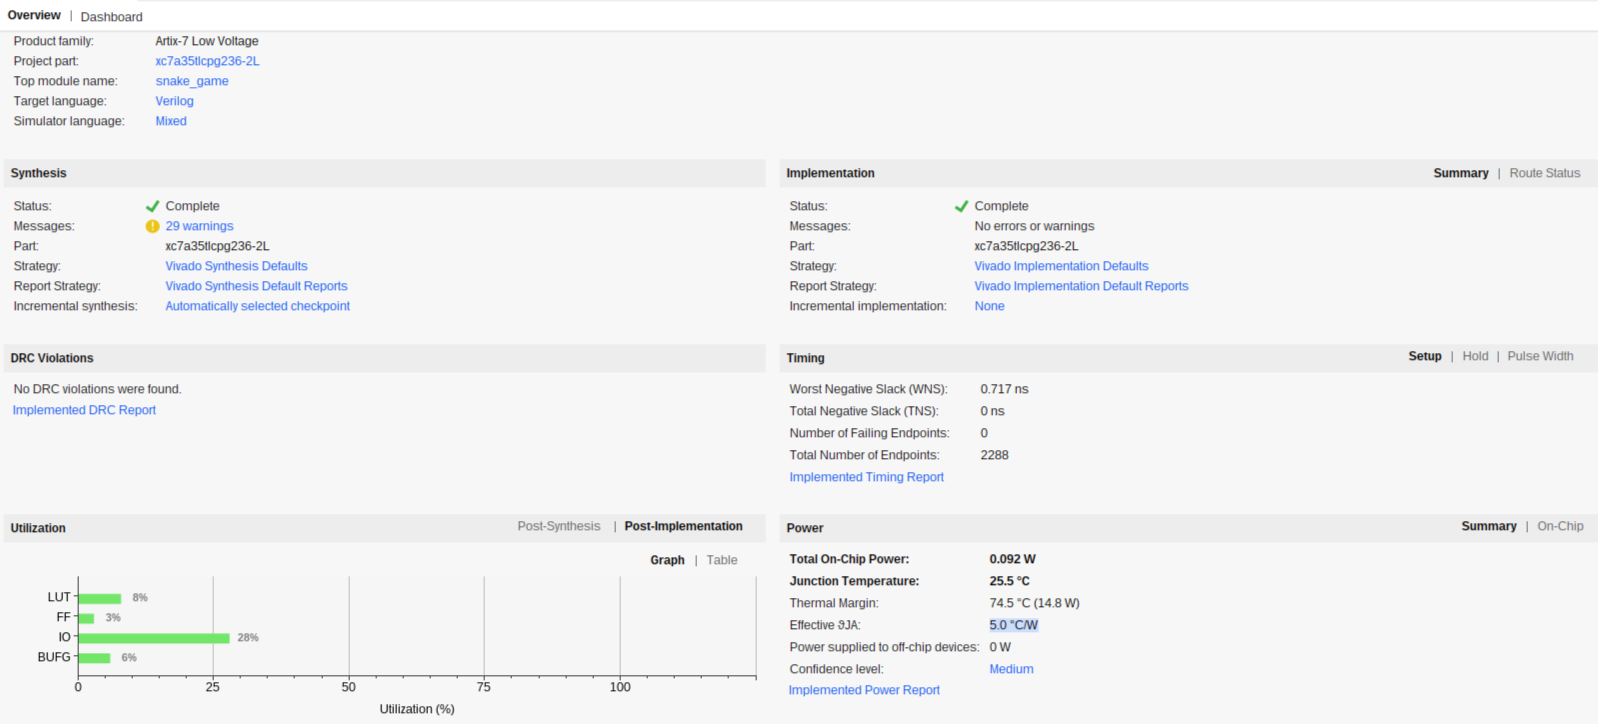
\includegraphics[width=\textwidth]{sum.png}
  \caption{Project dashboard: device, synthesis/implementation status,
  timing, utilization and power at a glance.}
\end{figure}

\subsection{Resource utilization}
\begin{figure}[H]\centering
  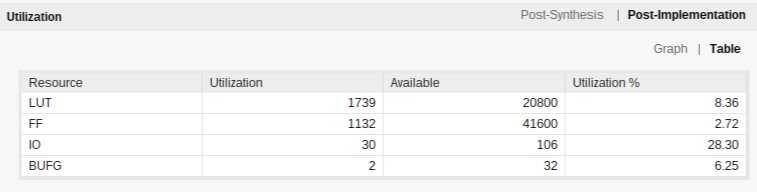
\includegraphics[width=0.85\textwidth]{utilizition.png}
  \caption{Post-implementation utilization on the \texttt{xc7a35t}.}
\end{figure}

\subsection{Timing}
\begin{figure}[H]\centering
  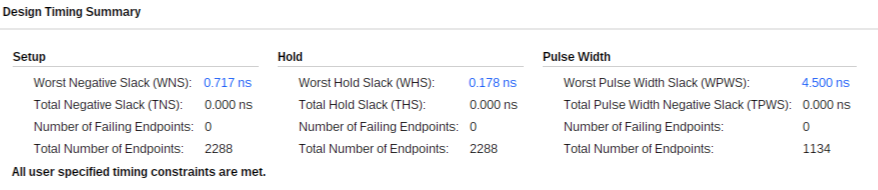
\includegraphics[width=\textwidth]{timing.png}
  \caption{Design timing summary --- WNS $=0.717$\,ns, all constraints met.}
\end{figure}

\begin{figure}[H]\centering
  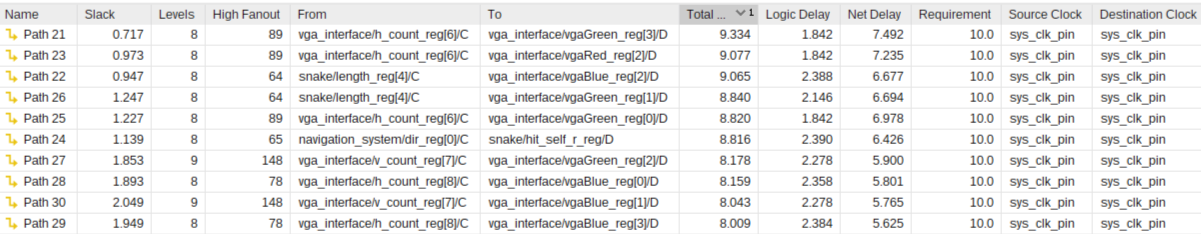
\includegraphics[width=\textwidth]{Critical.png}
  \caption{Worst (critical) paths report.}
\end{figure}

\subsection{Power}
\begin{figure}[H]\centering
  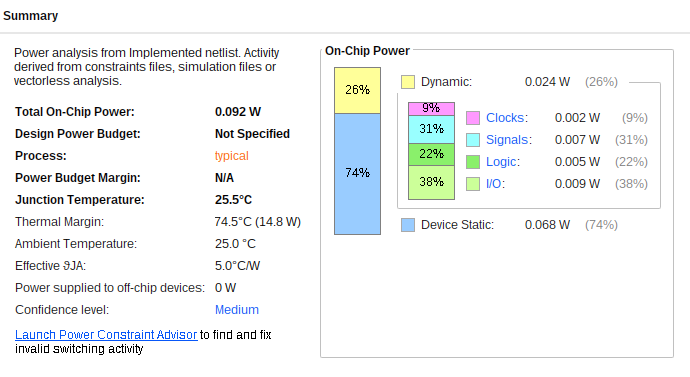
\includegraphics[width=0.8\textwidth]{power.png}
  \caption{On-chip power estimate --- total $0.092$\,W.}
\end{figure}

\subsection{Device view}
\begin{figure}[H]\centering
  
\includegraphics[height=9.5cm]{device.png}
  \caption{Implemented design placed and routed on the device.}
\end{figure}

\subsection{Schematics}
\begin{figure}[H]\centering
  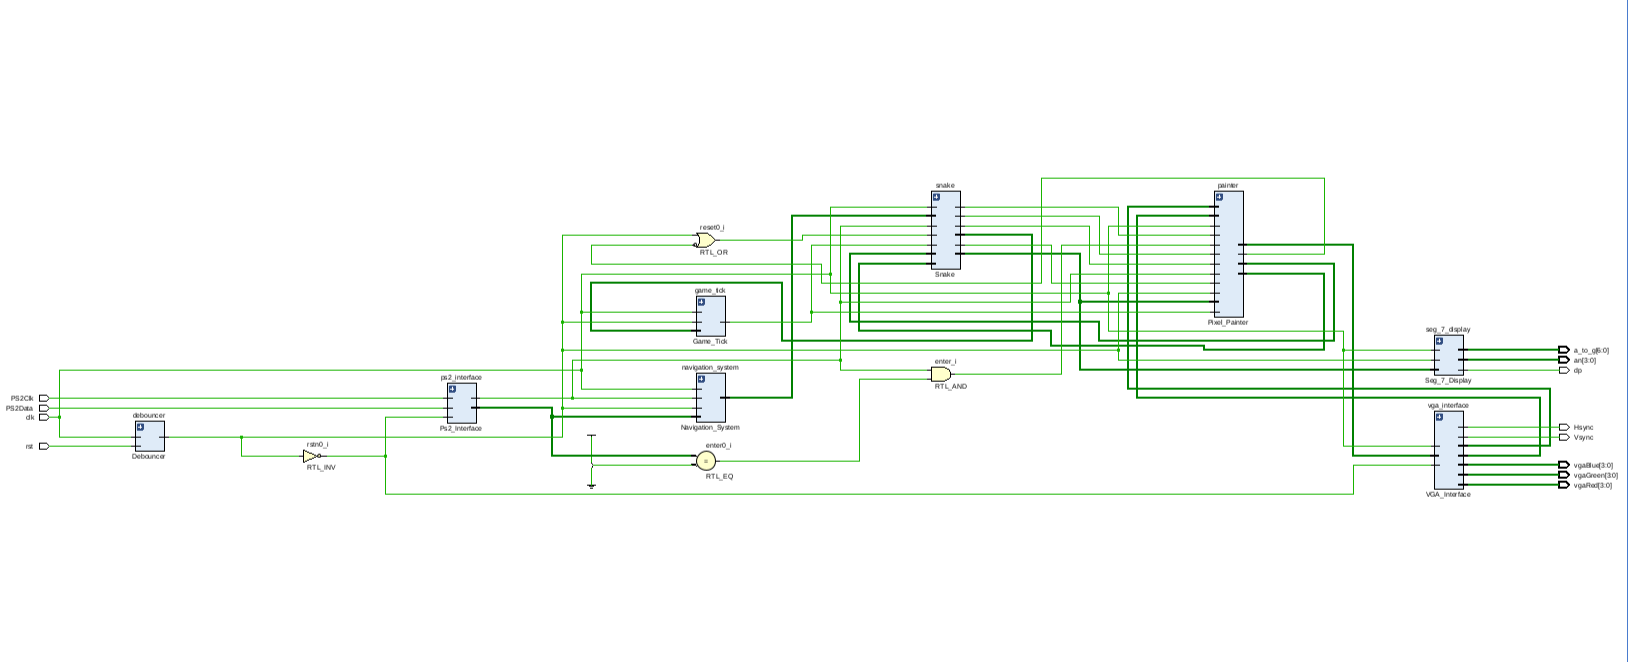
\includegraphics[width=\textwidth]{rtl_schematic.png}
  \caption{Elaborated RTL schematic (module-level view).}
\end{figure}

\begin{figure}[H]\centering
  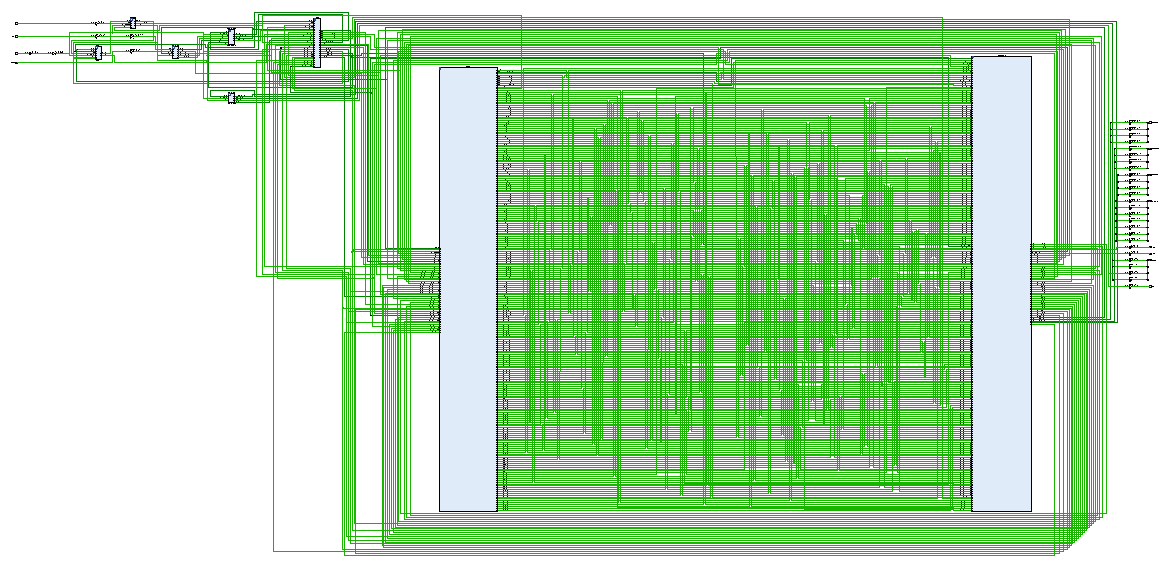
\includegraphics[width=\textwidth]{netlist_schematic_flip.pdf}
  \caption{Synthesised netlist schematic (full design).}
\end{figure}

% =====================================================================
\section{Results}
% =====================================================================
\subsection{Final state of the game}
The game is fully functional in simulation and on the board: it boots to
the welcome splash, any key starts a round, the snake moves at 7\,Hz and
accelerates with every food item, the score counts up on the 7-segment
display, reversal attempts are ignored, and hitting a wall or the body
freezes play and shows the skull game-over screen (bonus requirement),
from which a key press returns to the welcome screen. The simulated
scenario in \texttt{snake\_game\_tb} reproduces this full lifecycle.

\subsection{Photos of the game in action}
A full round on the monitor, from start to game over, is shown in
Figure~\ref{fig:sequence}.

\begin{figure}[H]\centering
  \begin{minipage}{0.485\textwidth}\centering
    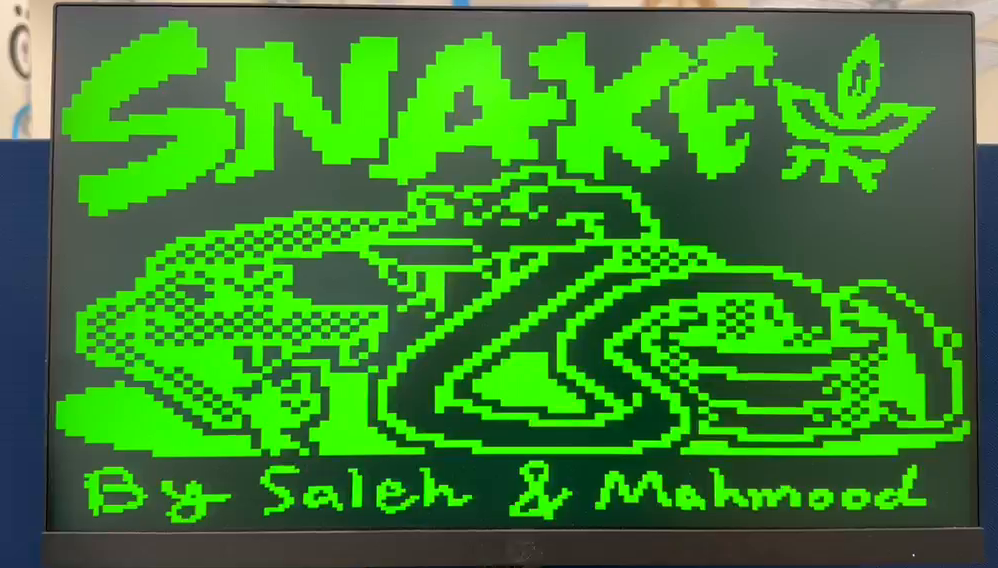
\includegraphics[width=\linewidth]{photo_welcome.png}\\[3pt]
    \small (a) Welcome / start screen
  \end{minipage}\hfill
  \begin{minipage}{0.485\textwidth}\centering
    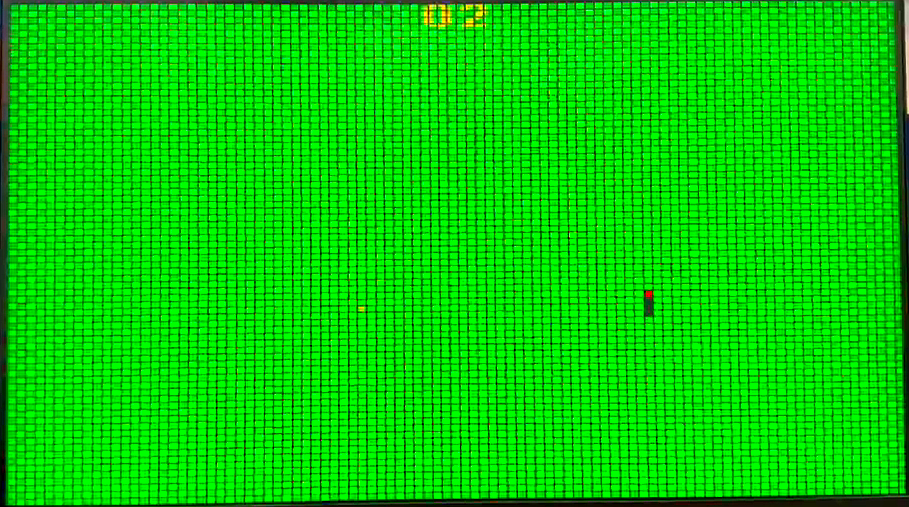
\includegraphics[width=\linewidth]{photo_play1.png}\\[3pt]
    \small (b) Playing --- snake and red food
  \end{minipage}

  \vspace{10pt}
  \begin{minipage}{0.485\textwidth}\centering
    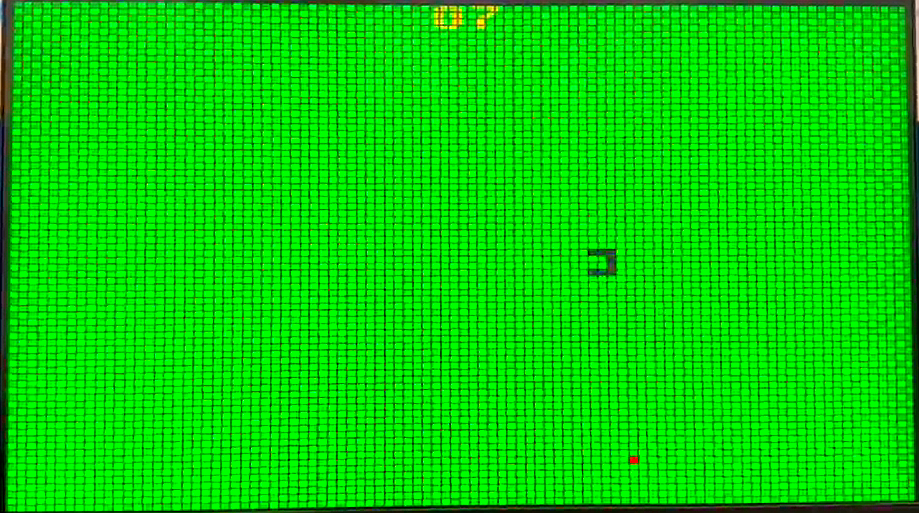
\includegraphics[width=\linewidth]{photo_play2.png}\\[3pt]
    \small (c) Later in the round --- longer snake
  \end{minipage}\hfill
  \begin{minipage}{0.485\textwidth}\centering
    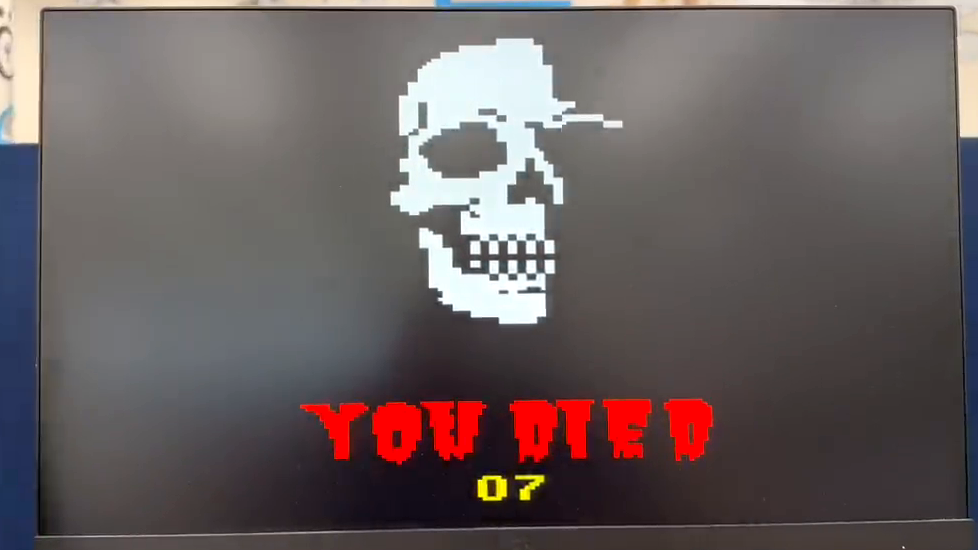
\includegraphics[width=\linewidth]{photo_gameover.png}\\[3pt]
    \small (d) Game over --- ``YOU DIED''
  \end{minipage}
  \caption{The Snake game running on the monitor: start, play, and the
  game-over screen after the snake collides.}
  \label{fig:sequence}
\end{figure}

\subsection{Demonstration video}
A video of the game running on the Basys3 board is available on YouTube:
\begin{center}
  \large\href{\youtubelink}{\texttt{\youtubelink}}\\[4pt]
  \normalsize\textcolor{red!60!black}{[REPLACE THE LINK ABOVE --- set
  \texttt{\textbackslash youtubelink} at the top of this file to your YouTube URL]}
\end{center}

% =====================================================================
\section{Problems Encountered and Solutions}\label{sec:problems}
% =====================================================================
\begin{enumerate}
  \item \textbf{Debouncer X-propagation in simulation.} The debouncer's
  hysteresis counter has no reset, so in simulation it powers up as
  \texttt{X} and the internal reset pulse never resolves (on the FPGA
  the global reset initialises it). \emph{Solution:} the integration
  testbench forces the internal \texttt{reset} net directly for a few
  cycles instead of pressing the button.

  \item \textbf{The real game tick is far too slow to simulate.} At
  7\,Hz, one snake step takes $14.3$ million clocks. \emph{Solution:}
  \texttt{snake\_game\_tb} generates its own fast tick (every 500
  clocks) and forces it onto the internal \texttt{tick} net, so a whole
  game fits in a short simulation.

  \item \textbf{Keyboard break codes re-triggered keys.} A PS/2 key
  release sends \texttt{F0} + scancode, which naively looks like a
  second key press. \emph{Solution:} the receiver skips
  \texttt{E0}/\texttt{F0} bytes and re-arms on the byte following
  \texttt{F0}, so exactly one \texttt{keyPressed} fires per physical
  press.

  \item \textbf{Timing warnings from a divided pixel clock.} Driving
  logic from a register-divided 50\,MHz clock produced ``non-clocked
  sequential cell'' critical warnings in Vivado. \emph{Solution:} the
  VGA module was restructured to run at 100\,MHz with a \texttt{pix\_en}
  clock-enable every second cycle -- one clock domain, no derived
  clocks.

  \item \textbf{Long combinational paths in the body scan.} Comparing
  the next head against all 64 body slots combinationally, directly at
  the tick, created long paths. \emph{Solution:} the next-head
  coordinates, self-hit and eat flags are registered one cycle before
  the movement update consumes them (\texttt{next\_x\_r},
  \texttt{hit\_self\_r}, \texttt{is\_eaten\_r}).

  \item \textbf{Food generator bias.} The coverage run
  (Figure~\ref{fig:coverage}) exposed the modulo bias of the LFSR
  mapping. Rather than adding a rejection loop, the bias was measured,
  shown to leave every cell reachable, and accepted; keyboard entropy
  was mixed into the LFSR feedback to decorrelate games.

  \item \placeholderbox{2.4cm}{Any additional problems encountered
  during the in-lab session and their solutions.}
\end{enumerate}

% =====================================================================
\section{Conclusion}
% =====================================================================
The experiment achieved all mandatory requirements and the bonus: a
playable, accelerating Snake game with VGA graphics, keyboard control,
hardware score display, and dedicated welcome and game-over screens. The
design cleanly separates reused interface blocks from the new game
logic, is parametric in the grid size and game speed, and was verified
bottom-up -- unit testbenches for the new generator modules, a coverage
analysis for the food placement, and a full-game integration testbench
that walks the complete IDLE $\rightarrow$ PLAY $\rightarrow$
GAME\_OVER lifecycle.

\end{document}
